% ============================================================================
% Knowledge-Based System Adaptif untuk Perhitungan PPh 21 dengan Akuisisi
% Pengetahuan Berbantuan LLM dari Regulasi dan Kebijakan Perusahaan
%
% Format : IEEEtran (journal)
% Bahasa : Indonesia; istilah teknis asing ditulis miring lewat \en{}
% Kompilasi: pdflatex, bibtex, lalu pdflatex dua kali (di folder paper/draft/)
% Sumber angka: docs/BAHAN_PAPER.md dan berkas hasil yang dirujuknya.
% ============================================================================
\documentclass[journal,a4paper]{IEEEtran}
\usepackage[T1]{fontenc}
\usepackage[english,indonesian]{babel}
\usepackage{cite}
\usepackage{amsmath,amssymb,amsfonts,amsthm,mathtools}
\usepackage{graphicx}
\usepackage{booktabs}
\usepackage{tabularx}
\usepackage{array}
\usepackage{multirow}
\usepackage{enumitem}
\usepackage{algorithm}
\usepackage{algpseudocode}
\usepackage{xcolor}
\usepackage{tikz}
\usetikzlibrary{positioning,arrows.meta,fit,calc}
\usepackage{url}
\usepackage[hidelinks]{hyperref}

\newcolumntype{L}{>{\raggedright\arraybackslash}X}
\newcolumntype{P}[1]{>{\raggedright\arraybackslash}p{#1}}

% Istilah asing (tidak diterjemahkan) ditulis miring.
% Bentuk miring dipilih langsung agar tetap miring di judul berhuruf kapital kecil.
\makeatletter
\DeclareRobustCommand{\en}[1]{{\usefont{\f@encoding}{\f@family}{\f@series}{it}#1\/}}
\makeatother

% Penamaan dalam Bahasa Indonesia
\renewcommand{\IEEEkeywordsname}{Kata Kunci}
\addto\captionsindonesian{\renewcommand{\refname}{Daftar Pustaka}\renewcommand{\abstractname}{Abstrak}%
  \renewcommand{\figurename}{Gambar}\renewcommand{\tablename}{Tabel}}
\floatname{algorithm}{Algoritma}
\newtheorem{definisi}{Definisi}

% Notasi: x = kasus uji, t = masa pajak, \omega = tanggal pengetahuan,
% m = jumlah kandidat, c = jumlah kandidat benar, n = indeks peristiwa.
\newcommand{\K}{\mathcal{K}}
\newcommand{\hasil}{\mathit{hasil}}
\newcommand{\emas}{\star}
\newcommand{\SG}{S^{G}}
\newcommand{\SE}{S^{E}}

\tikzset{
  kotakalur/.style={draw, rounded corners=2pt, align=center, font=\scriptsize, inner sep=3pt, minimum height=0.6cm},
  kotakdata/.style={draw, align=center, font=\scriptsize, inner sep=3pt, minimum height=0.6cm, fill=gray!10},
  panah/.style={-{Stealth[length=2mm]}, semithick},
  label/.style={font=\tiny, align=center}
}

\begin{document}
\title{\en{Knowledge-Based System} Adaptif untuk Perhitungan PPh 21 dengan Akuisisi Pengetahuan Berbantuan LLM dari Regulasi dan Kebijakan Perusahaan}
\author{Obi Kastanya}
\maketitle

\begin{abstract}
Perhitungan PPh Pasal 21 harus mengikuti perubahan regulasi dan kebijakan perusahaan, tetapi aturannya umumnya tertanam di kode. Penelitian formalisasi pajak berbantuan LLM membangun basis aturan dari nol untuk satu keadaan hukum, sehingga belum diketahui apakah pembaruan berulang menjaga hasil periode lama dan apakah kesalahan merambat. Penelitian ini mengusulkan \en{knowledge-based system} dengan \en{knowledge base} bitemporal dua lapis, yaitu regulasi dan kebijakan perusahaan, serta akuisisi pengetahuan inkremental berbantuan LLM. Setiap pembaruan diperiksa lima gerbang verifikasi, kandidat dipilih lewat konsensus perilaku, dan sistem \en{abstain} bila tidak yakin. Evaluasinya memutar ulang 13 perubahan regulasi PPh 21 nyata 2023--2026 beserta 20 pengecoh dan menguji 16 perubahan yang tidak dilihat perancang. Rancangan inti didaftarkan sebelum eksperimen, sedangkan ablasi, model kedua, dan rantai pembangkitan ulang ditambahkan lewat amandemen sesudah hasil awal terlihat. Emas dan perubahan uji hanya ditinjau agen AI independen, bukan pakar manusia. Representasi menyatakan 16 dari 16 perubahan tak terlihat tanpa mengubah \en{engine} (batas bawah satu sisi 95\% 0,829), dengan syarat konvensi pembulatan contoh diselaraskan. Pada 18 dokumen nyata, pembaruan salah tanpa terdeteksi terjadi pada 3 dokumen (batas atas 0,377, di atas ambang 0,25) dan pembaruan benar pada 8 (CI 0,22--0,69). Pada mode berantai, 31 dari 33 peristiwa tidak menambah kesalahan baru (batas bawah 0,821), tetapi pada rantai yang dibangkitkan ulang hanya 23 dari 33 (batas bawah 0,540). \en{Recall} deteksi dampak lintas lapis 0,91 (CI 0,75--1,00).
\end{abstract}

\begin{IEEEkeywords}
Akuisisi pengetahuan, \en{knowledge-based system}, \en{knowledge graph}, \en{large language model}, perubahan regulasi, PPh Pasal 21, \en{rules as code}
\end{IEEEkeywords}

% ============================================================================
\section{Pendahuluan}
\label{sec:pendahuluan}
% ============================================================================
\IEEEPARstart{P}{Ph} Pasal 21 dipotong setiap bulan dari penghasilan pegawai, sehingga kesalahan perhitungan langsung memengaruhi setiap slip gaji. Regulasinya sering berubah. Dalam empat tahun pajak 2023--2026, korpus penelitian ini mencatat 13 peristiwa yang mengubah perhitungan PPh 21 pegawai tetap (Tabel~\ref{tab:korpus}), tujuh di antaranya terbit pada 2025. Jenisnya beragam: nilai parameter seperti batas upah iuran Jaminan Pensiun, klasifikasi penghasilan seperti natura, fasilitas Pajak Ditanggung Pemerintah (DTP) dengan kriteria sektor, aturan pembulatan yang berlaku surut, dan pada 2024 pergantian metode perhitungan ke tarif efektif rata-rata (TER)~\cite{pp58_2023,pmk168_2023}.

Pada praktik saat ini, aturan pajak dan kebijakan \en{payroll} tertanam bercampur di kode atau \en{spreadsheet}~\cite{ramadhani2021grossup,yulistyawati2022payroll,kusuma2026pph21}. Akibatnya ada tiga masalah. Pertama, setiap perubahan regulasi menuntut pemrograman ulang. Sebagai ilustrasi dari dua repositori, di antara kalkulator PPh 21 sumber terbuka yang sudah ada sebelum PP 58/2023, satu memasukkan TER 26 hari sesudah peraturan terbit dan satu lagi baru 915 hari sesudahnya (Bagian~\ref{subsec:hasil-rq3}). Kedua, tidak ada bukti bahwa perubahan itu tidak menggeser hasil periode lama. Ketiga, kebijakan perusahaan yang menjadi melanggar setelah regulasi berubah tidak terdeteksi.

\en{Knowledge-based system} (KBS) memisahkan pengetahuan dari kode~\cite{mowbray2023scaling,merigoux2021catala}, tetapi memindahkan beban ke pemeliharaan \en{knowledge base}. Inilah \en{knowledge acquisition bottleneck}. Metode akuisisi inkremental seperti \en{Ripple-Down Rules} sudah lama ada, tetapi tetap membutuhkan pakar manusia untuk setiap perubahan~\cite{compton2021rdr}.

\en{Large language model} (LLM) dapat menerjemahkan teks hukum menjadi aturan terstruktur~\cite{janatian2023texttostructure,makowski2025dmn}, tetapi tidak andal untuk perhitungan yang menuntut ketepatan dan dapat mengarang isi hukum~\cite{blairstanek2023gpt3,nay2024taxattorneys,dahl2024legalfictions}. Penelitian formalisasi pajak berbantuan LLM membangun basis aturan dari nol untuk keadaan hukum pada satu waktu. Penelitian penyuntingan pengetahuan LLM menunjukkan bahwa suntingan berurutan dapat merusak pengetahuan lama~\cite{gupta2024editing}. Sejauh penelusuran kami, belum ada penelitian yang mengukur tiga hal pada basis aturan yang dieksekusi: apakah pembaruan berulang dari LLM menjaga hasil periode lama, apakah kesalahan merambat dari satu perubahan ke perubahan berikutnya, dan bagaimana dampaknya terhadap lapisan kebijakan perusahaan.

Penelitian ini mengusulkan KBS yang pengetahuannya disimpan sebagai \en{knowledge graph} bitemporal dua lapis dan dijalankan \en{inference engine} deterministik (Gambar~\ref{fig:ikhtisar}). LLM tidak menghitung pajak. LLM hanya membaca dokumen regulasi atau kebijakan dan menyusun beberapa kandidat pembaruan $\Delta$. Lima gerbang verifikasi menyaring kandidat, konsensus perilaku memilih satu, dan sistem \en{abstain} bila tidak ada kandidat yang meyakinkan. Analisis dampak statis atas graf melaporkan kebijakan perusahaan yang terdampak.

\begin{figure}[t]
\centering
\begin{tikzpicture}[node distance=6mm and 6mm]
\node[kotakdata, text width=2.2cm] (dok) {Dokumen regulasi atau kebijakan};
\node[kotakalur, right=of dok, text width=2.6cm] (llm) {LLM: relevansi berkutipan, $m$ kandidat $\Delta$};
\node[kotakalur, below=of llm, text width=2.6cm] (gerbang) {Gerbang G1--G5 dan satu putaran perbaikan};
\node[kotakalur, left=of gerbang, text width=2.2cm] (kons) {Konsensus perilaku atau \en{abstain}};
\node[kotakdata, below=of kons, text width=2.2cm] (kb) {\en{Knowledge base} bitemporal dua lapis (graf RDF)};
\node[kotakalur, right=of kb, text width=2.6cm] (eng) {\en{Inference engine}: nilai PPh 21 dan jejak sampai pasal};
\node[kotakalur, below=of kb, text width=2.2cm] (dampak) {Analisis dampak lintas lapis (SPARQL)};
\node[kotakdata, right=of dampak, text width=2.6cm] (rev) {Peninjau manusia};
\draw[panah] (dok) -- (llm);
\draw[panah] (llm) -- (gerbang);
\draw[panah] (gerbang) -- (kons);
\draw[panah] (kons) -- node[label, left]{$\hat{\Delta}$} (kb);
\draw[panah] (kb) -- (eng);
\draw[panah] (kb) -- (dampak);
\draw[panah] (dampak) -- (rev);
\draw[panah, dashed] (kb.north east) -- (gerbang.south west);
\end{tikzpicture}
\caption{Ikhtisar sistem. LLM hanya menyusun kandidat pembaruan. Perhitungan dijalankan \en{engine} deterministik atas \en{knowledge base}. Garis putus-putus menunjukkan KB yang menjadi konteks LLM dan basis gerbang.}
\label{fig:ikhtisar}
\end{figure}

Penelitian ini menjawab empat pertanyaan penelitian.
\begin{enumerate}[label=\textbf{RQ\arabic*},leftmargin=*,nosep]
  \item \textbf{Adaptivitas representasi.} Sejauh mana representasi pengetahuan temporal dua lapis dapat menyatakan perubahan regulasi dan kebijakan, termasuk jenis perubahan yang tidak diketahui saat representasi dirancang, tanpa mengubah kode \en{engine}?
  \item \textbf{Akuisisi satu langkah.} Seberapa sering akuisisi berbantuan LLM menerapkan pembaruan yang benar, seberapa sering ia menerapkan pembaruan salah tanpa terdeteksi, dan berapa besar peran gerbang verifikasi pada kedua angka itu?
  \item \textbf{Adaptivitas operasional berantai.} Pada rangkaian perubahan regulasi yang nyata, berapa peristiwa yang berhasil diterapkan otomatis, dan apakah kesalahan merambat dari satu peristiwa ke peristiwa berikutnya?
  \item \textbf{Dampak lintas lapis.} Seberapa lengkap dan tepat sistem mengidentifikasi kebijakan perusahaan yang terdampak atau menjadi melanggar setelah regulasi berubah?
\end{enumerate}

Kontribusinya sebagai berikut.
\begin{enumerate}[label=\textbf{K\arabic*},leftmargin=*,nosep]
  \item Representasi pengetahuan temporal dua lapis untuk perhitungan pajak penghasilan pegawai, dengan resolusi konflik antarlapis dan analisis dampak lintas lapis (RQ1, RQ4).
  \item Metode akuisisi pengetahuan inkremental berbantuan LLM dengan gerbang verifikasi, gerbang non-vakuitas, dan pemilihan kandidat berbasis konsensus perilaku (RQ2).
  \item Definisi adaptivitas representasional dan operasional, serta protokol \en{regulation replay} yang memisahkan kesalahan bawaan, kesalahan baru, dan kesalahan yang dipicu perambatan, beserta bukti empiris pada rangkaian perubahan PPh 21 yang nyata (RQ3).
  \item Artefak berupa \en{knowledge base}, korpus perubahan beserta pembaruan emas, \en{test suite} dengan \en{ground truth}, dan kode evaluasi.
\end{enumerate}
Tabel~\ref{tab:lacak} menghubungkan setiap kontribusi dengan RQ, hipotesis, dan metrik utamanya.

Bagian~\ref{sec:masalah} menjelaskan domain dan merumuskan masalah. Bagian~\ref{sec:terkait} membahas penelitian terkait. Bagian~\ref{sec:representasi} dan~\ref{sec:akuisisi} menjelaskan representasi dan metode akuisisi. Bagian~\ref{sec:evaluasi} menjelaskan metodologi evaluasi, Bagian~\ref{sec:hasil} melaporkan hasil, Bagian~\ref{sec:pembahasan} membahasnya, dan Bagian~\ref{sec:kesimpulan} menutup penelitian ini.

% ============================================================================
\section{Latar belakang dan rumusan masalah}
\label{sec:masalah}
% ============================================================================
\subsection{Perhitungan PPh 21 pegawai tetap}
PPh 21 pegawai tetap dihitung dari penghasilan bruto, yaitu gaji, tunjangan, penghasilan tidak teratur seperti THR dan bonus, premi jaminan sosial yang dibayar pemberi kerja, dan sejak Juli 2023 natura. Bruto dikurangi biaya jabatan dan iuran pegawai yang menjadi pengurang, lalu penghasilan tidak kena pajak (PTKP) menurut status, sehingga diperoleh penghasilan kena pajak (PKP). Atas PKP setahun dikenakan tarif progresif Pasal 17~\cite{uu7_2021,pmk101_2016}. Sampai 2023, PPh setiap masa dihitung dengan menyetahunkan penghasilan~\cite{per16_2016}. Sejak 2024, masa Januari sampai November memakai TER bulanan, yaitu tarif atas bruto bulanan menurut kategori A, B, atau C yang ditentukan status PTKP. Pada masa pajak terakhir, pajak setahun dihitung ulang dengan tarif Pasal 17 dan dikurangi potongan masa sebelumnya~\cite{pp58_2023,pmk168_2023}. Fasilitas DTP 2025--2026 menambah kriteria sektor dan batas penghasilan~\cite{pmk10_2025,pmk72_2025,pmk105_2025}. Tabel~\ref{tab:ruang-pajak} merangkum dimensi yang menentukan besarnya pajak.

\begin{table}[t]
\centering
\caption{Dimensi perhitungan PPh 21 pegawai tetap yang dicakup}
\label{tab:ruang-pajak}
\scriptsize
\begin{tabularx}{\columnwidth}{@{}P{2.0cm} L@{}}
\toprule
\textbf{Dimensi} & \textbf{Nilai} \\
\midrule
Rezim & Disetahunkan (sampai 2023); TER (sejak 2024); TER dengan fasilitas DTP (2025--2026) \\
Lapisan Pasal 17 & 5\%, 15\%, 25\%, 30\%, 35\% (4 lapisan sebelum UU HPP) \\
Kategori TER & A (44 lapisan), B (40), C (41), menurut lampiran PP 58/2023 \\
Status PTKP & TK/0--TK/3, K/0--K/3; menentukan kategori TER \\
Metode & \en{Gross}, \en{gross-up}, ditanggung pemberi kerja \\
Pola kerja & Setahun penuh, masuk di tengah tahun, keluar di tengah tahun \\
Penghasilan & Teratur, tidak teratur (THR, bonus), natura, premi BPJS, zakat lewat pemberi kerja \\
\bottomrule
\end{tabularx}
\end{table}

Ruang lingkupnya adalah pegawai tetap pada pemberi kerja swasta atau BUMN, tahun pajak 2023--2026 untuk data uji dan tahun sebelumnya untuk data pengembangan. Pegawai tidak tetap, bukan pegawai, pensiunan, ASN, peserta magang, PPh 26, dan pegawai di IKN berada di luar lingkup. Batasan antardimensi ikut menentukan ruang uji. Contohnya, status PTKP menentukan kategori TER, dan fasilitas DTP hanya ada sejak 2025.

\subsection{Kebijakan perusahaan dan batas kewenangannya}
Perusahaan menentukan komponen penghasilan seperti prorata, THR, tunjangan, lembur, siapa yang menanggung pajak, dan pembagian iuran. Pilihan yang memang diserahkan kepada perusahaan, misalnya metode \en{gross}, \en{gross-up}, atau ditanggung pemberi kerja, bukan konflik. Perusahaan tidak boleh menyimpangi ketentuan wajib, misalnya klasifikasi jenis penghasilan atau penerusan fasilitas pemerintah kepada pegawai. Contoh konflik nyata ada pada PKB PT Wijaya Karya 2025--2026 Pasal 22 ayat (3), yang menyatakan insentif pajak pemerintah tidak diberikan kepada pegawai. Ketentuan ini berlawanan dengan PMK 10/2025 Pasal 5 ayat (1), yang mewajibkan PPh DTP dibayarkan tunai kepada pegawai~\cite{pmk10_2025}. Konflik ini laten, karena perusahaan itu bukan sektor penerima DTP. Taksonomi konflik penelitian ini memuat sepuluh jenis (C1--C10), misalnya klasifikasi menyimpang (C1), parameter usang (C6), dan hak minimum dilanggar (C10). Konflik yang diukur RQ4 adalah konflik \emph{terpicu perubahan}, yaitu kebijakan yang tadinya sah menjadi berkonflik setelah regulasi berubah.

\subsection{Jenis perubahan regulasi}
\label{subsec:jenis-perubahan}
Taksonomi perubahan disusun sebelum ada keluaran LLM. Setiap peristiwa diberi satu jenis utama: parameter (T1), tabel tarif (T2), klasifikasi penghasilan (T3), fasilitas baru (T4), perubahan cakupan (T5), perubahan masa (T6), pergantian metode (T7), pencabutan tanpa pengganti (T8), perubahan prosedur hitung seperti pembulatan (T9), dan perubahan kebijakan perusahaan (T10). Sifat tambahannya adalah berlaku surut (S1), bersyarat (S2), sementara (S3), terdiri atas beberapa dokumen (S4), mengubah dokumen lain (S5), dan bergantung tabel lampiran (S6). Pengecoh juga diberi jenis, misalnya ketentuan administrasi (X1) dan subjek di luar lingkup (X2). Hasil dilaporkan per jenis, sehingga jenis mudah seperti parameter tidak digabung dengan jenis struktural.

\subsection{Rumusan masalah}
Masukannya adalah sistem yang benar untuk keadaan hukum sebelum suatu perubahan, beserta dokumen perubahan itu. Keluarannya adalah sistem yang benar untuk keadaan hukum sesudahnya, tanpa perubahan kode dan tanpa perubahan pada hasil yang tidak seharusnya berubah. Definisi formalnya ada di Bagian~\ref{subsec:adaptif}.

% ============================================================================
\section{Penelitian terkait}
\label{sec:terkait}
% ============================================================================
\subsection{\en{Rules as code} dan formalisasi peraturan pajak}
Catala menerjemahkan teks undang-undang ke bahasa pemrograman dengan pola kasus umum dan pengecualian berbasis \en{default logic}, dan evaluasinya menemukan \en{bug} pada implementasi resmi~\cite{merigoux2021catala,huttner2022catala}. Mlang menggantikan \en{compiler} warisan mesin pajak penghasilan Prancis~\cite{merigoux2021mlang}. Ekosistem yang sama memformalkan aritmetika tanggal~\cite{monat2024date} dan membangkitkan kasus uji dengan \en{concolic execution}~\cite{goutagny2025cutecat}. DataLex~\cite{mowbray2023scaling,mowbray2023xai}, Logical English~\cite{kowalski2022logicalenglish}, dan OpenFisca mengikuti prinsip yang sama. Meessen menunjukkan bahwa banyak keputusan normatif dibuat di dalam komponen teknis~\cite{meessen2023arrows}, dan Witt dkk.\ membedakan validasi teknis dari kesesuaian hukum~\cite{witt2024encoding}. Untuk \en{payroll}, Dumancic dkk.\ menyatakan legislasi pajak dan jaminan sosial secara deklaratif untuk optimasi kebijakan~\cite{dumancic2021payroll}, dan Al-Hawari dkk.\ membangun sistem \en{payroll} berbasis aturan~\cite{alhawari2026payroll}. Di Indonesia, sistem PPh 21 umumnya prosedural~\cite{ramadhani2021grossup,yulistyawati2022payroll,kusuma2026pph21}, dan TER menimbulkan lebih bayar pada penghasilan tidak teratur~\cite{sherra2025ter}. Dalam semua karya ini pengetahuan ditulis manusia. Parameter berversi sudah ada, tetapi pembaruan oleh mesin belum dievaluasi.

\subsection{Akuisisi pengetahuan inkremental}
\en{Ripple-Down Rules} menambah aturan setiap kali pakar menemukan kasus yang salah, dan \en{cornerstone case} menjaga agar aturan baru tidak merusak kasus yang sudah benar~\cite{compton2021rdr}. Gerbang regresi G4 dalam penelitian ini setara dengan \en{cornerstone case}. Pada sisi logika hukum, perubahan hukum dan revisi teori dirumuskan dengan operator revisi berwaktu~\cite{moguillansky2024temporalised}, revisi \en{defeasible logic} terbukti sulit secara komputasi~\cite{olivieri2025revising}, dan konsekuensi janggal dapat ditelusuri ke aturan penyebabnya~\cite{fungwacharakorn2021debugging}. Dalam kelompok ini pakar manusia tetap menulis setiap perubahan.

\subsection{LLM untuk formalisasi hukum dan pajak}
Kelompok ini paling dekat dengan penelitian ini. LLM dipakai untuk mengubah teks hukum menjadi struktur yang mendukung sistem pakar hukum~\cite{janatian2023texttostructure}, untuk menyusun aturan DMN bagi kantor akuntan~\cite{makowski2025dmn}, dan untuk menurunkan relasi metamorfik bagi perangkat lunak pajak~\cite{srinivas2023fewshot,khiabani2026agentic}. Kemampuan LLM menerapkan hukum pajak meningkat antargenerasi, tetapi belum setara ahli~\cite{blairstanek2023gpt3,nay2024taxattorneys}, dan alat riset hukum komersial masih berhalusinasi~\cite{magesh2025hallucination}. Karya-karya ini memformalkan dari nol untuk keadaan hukum pada satu waktu.

\subsection{Pembaruan berulang oleh LLM dan evaluasinya}
Penyuntingan pengetahuan LLM secara berurutan merusak kemampuan model setelah banyak suntingan~\cite{gupta2024editing}. Evaluasi berbasis eksekusi dengan $n$ kandidat dan pemilihan satu jawaban, yang dikenal sebagai \en{n@k}, berasal dari pembangkitan kode~\cite{li2022alphacode}. Prediksi selektif memungkinkan model menahan jawaban ketika tidak yakin, dan kinerjanya diukur sebagai pasangan risiko dan cakupan~\cite{xin2021abstention}. Ketiganya menjadi dasar metrik RQ2 dan RQ3. Metrik tersebut belum diterapkan pada basis aturan hukum yang dieksekusi dan berversi waktu.

\subsection{Representasi temporal dan \en{knowledge graph} hukum}
De Martim memodelkan norma sebagai karya dengan ekspresi berversi agar jawaban tidak anakronistik~\cite{demartim2025satgraph}, dan Kharraz dkk.\ mendefinisikan konflik pada logika normatif berwaktu~\cite{kharraz2024conflicts}. Penelitian ini memakai ulang standar ELI, OWL-Time, dan PROV-O untuk dokumen, masa berlaku, dan provenans.

\subsection{Konflik norma, verifikasi \en{knowledge base}, dan pengujian perangkat lunak pajak}
Deteksi konflik norma~\cite{robaldo2024compliance,khoja2026consistency}, anomali \en{rule base}~\cite{boujelben2025anomalies}, dan pengujian perangkat lunak pajak yang sulit karena acuan kebenarannya tidak tersedia~\cite{tizpaz2023metamorphic,li2025mrgeneration} menjadi dasar rancangan \en{ground truth} penelitian ini. Demikian juga \en{property-based testing}~\cite{goldstein2024pbt,ravi2025pbtpython} dan \en{mutation analysis}~\cite{petrovic2022mutation,petrovic2021mutation}. Karya-karya tersebut dipakai sebagai dasar rancangan, bukan sebagai kontribusi.

Tabel~\ref{tab:posisi} merangkum posisi penelitian ini. Tanda ``--'' berarti aspek itu tidak dilaporkan sebagai fokus publikasi yang dirujuk.

\begin{table*}[t]
\centering
\caption{Posisi penelitian terhadap karya terkait}
\label{tab:posisi}
\scriptsize
\begin{tabularx}{\textwidth}{@{}P{2.9cm} P{1.9cm} L P{1.9cm} P{1.4cm} P{1.5cm} P{1.3cm} P{2.3cm}@{}}
\toprule
\textbf{Karya} & \textbf{Domain} & \textbf{Representasi} & \textbf{Penyusun pengetahuan} & \textbf{Pembaruan inkremental} & \textbf{Perambatan kesalahan diukur} & \textbf{Lapisan perusahaan} & \textbf{Evaluasi} \\
\midrule
Catala~\cite{merigoux2021catala,huttner2022catala} & pajak dan tunjangan & DSL dengan \en{default logic} & manusia & -- & -- & -- & temuan \en{bug} implementasi resmi \\
DataLex~\cite{mowbray2023scaling,mowbray2023xai} & legislasi umum & bahasa aturan semi-alami dan \en{inference engine} & manusia & -- & -- & -- & -- \\
Dumancic dkk.~\cite{dumancic2021payroll} & \en{payroll} & representasi formal ke \en{constraint} & manusia & -- & -- & -- & pemakaian di lembaga jaminan sosial \\
\en{Ripple-Down Rules}~\cite{compton2021rdr} & umum & aturan dengan pengecualian & pakar manusia & ya & -- & -- & \en{cornerstone case} \\
Janatian dkk.~\cite{janatian2023texttostructure} & sistem pakar hukum & struktur dari teks & LLM & -- & -- & -- & penilaian manusia \\
Makowski \& Tr\k{a}bka~\cite{makowski2025dmn} & akuntansi pajak & DMN & AI generatif dan manusia & -- & -- & -- & studi kasus \\
De Martim~\cite{demartim2025satgraph} & norma hukum & graf norma berversi & -- & versi norma & -- & -- & -- \\
Sistem PPh 21 Indonesia~\cite{ramadhani2021grossup,yulistyawati2022payroll,kusuma2026pph21} & PPh 21 & aplikasi prosedural atau \en{spreadsheet} & manusia & -- & -- & -- & -- \\
\midrule
\textbf{Penelitian ini} & PPh 21 & \en{knowledge graph} temporal dua lapis dan aturan yang dapat dieksekusi & LLM dengan gerbang & ya & ya & ya & \en{regulation replay} \\
\bottomrule
\end{tabularx}
\end{table*}

% ============================================================================
\section{Representasi pengetahuan dan \en{inference engine}}
\label{sec:representasi}
% ============================================================================
\subsection{Model pengetahuan}
Pengetahuan struktural, yaitu dokumen dan pasal, aturan, parameter, tabel, konsep fakta, kebijakan, versi, dan relasi antarunsur, disimpan sebagai \en{knowledge graph} RDF/OWL dengan validasi SHACL dan kueri SPARQL. Pengetahuan komputasional berupa ekspresi perhitungan disimpan sebagai atribut aturan dan dijalankan \en{inference engine}. Asal-usul aturan dan ketergantungan kebijakan dijawab sebagai kueri graf tanpa menjalankan perhitungan, dan dipakai analisis dampak, G3, dan pemeriksa anomali. Aritmetika pajak menuntut ketepatan rupiah, pecahan eksak, dan iterasi titik tetap, yang tidak praktis dinyatakan sebagai \en{triple}. Dengan pembagian ini, perubahan regulasi hanya menyentuh data graf.

\begin{definisi}[\en{Knowledge base}]
\label{def:kb}
$\K = \langle \mathcal{O}, \mathcal{R}, \mathcal{P}, \mathcal{T}, \mathcal{C}, \mathcal{D} \rangle$ terdiri atas ontologi konsep, rekaman aturan, rekaman parameter berversi, versi tabel, batasan wajib, dan dokumen sumber beserta provenans pembaruan. Setiap unsur $\mathcal{R}$ berada pada lapisan $\ell \in \{\mathit{reg}, \mathit{prs}\}$. Parameter, tabel, dan batasan hanya ada di lapisan regulasi. Setiap aturan perusahaan milik tepat satu kebijakan $P_j$, sehingga $\K = \K_{\mathit{reg}} \oplus \bigcup_j P_j$, dan untuk kasus $x$ hanya kebijakan $P(x)$ yang disebut data kasus yang dipasang.
\end{definisi}

\begin{definisi}[Aturan]
\label{def:aturan}
Rekaman aturan $r = \langle \mathit{id}, \ell, \sigma, \kappa, [t_s, t_e], t_c, \varphi, f \coloneqq e, \mathit{ov}, \mathit{src} \rangle$ memuat identitas, lapisan, sifat $\sigma \in \{$wajib, \en{default}, opsional$\}$, lingkup $\kappa \in \{$masa, tahun$\}$, masa berlaku, tanggal pencatatan $t_c$ (tanggal terbit dokumen sumber), kondisi, fakta yang dihasilkan beserta ekspresinya, daftar aturan yang dikalahkannya, dan sumber berupa dokumen, pasal, dan kutipan. Rekaman tidak pernah disunting di tempat. Operasi \en{add}, \en{change}, dan \en{remove} menambah rekaman baru, dengan \en{remove} berupa rekaman nisan.
\end{definisi}

\begin{definisi}[Hasil perhitungan]
\label{def:hasil}
$\hasil(\K, x, t, \omega)$ adalah nilai fakta keluaran untuk kasus $x$ pada masa pajak $t$, dihitung dengan $\K_{\mathit{reg}}$ sebagaimana diketahui pada tanggal $\omega$ ditambah lapisan $P(x)$. Kasus adalah satu pegawai tetap pada satu pemberi kerja untuk satu tahun pajak. Fakta utama adalah PPh 21 terutang per masa. Fakta pendukung yang dinilai mencakup PPh DTP, bruto, tunjangan pajak, \en{take home pay}, premi dan iuran BPJS, dan fakta masa pajak terakhir. Selain nilai, \en{engine} mengeluarkan laporan konflik dan jejak setiap fakta.
\end{definisi}

Ontologi (Gambar~\ref{fig:ontologi}) memakai ulang ELI untuk dokumen dan pasal, OWL-Time untuk masa berlaku, dan PROV-O untuk provenans rekaman dan pembaruan. Setiap pembaruan disimpan sebagai satu \en{named graph} di \en{triple store} GraphDB, dan sidik jari SHA-256 setiap versi dicatat di graf metadata.

\begin{figure*}[t]
\centering
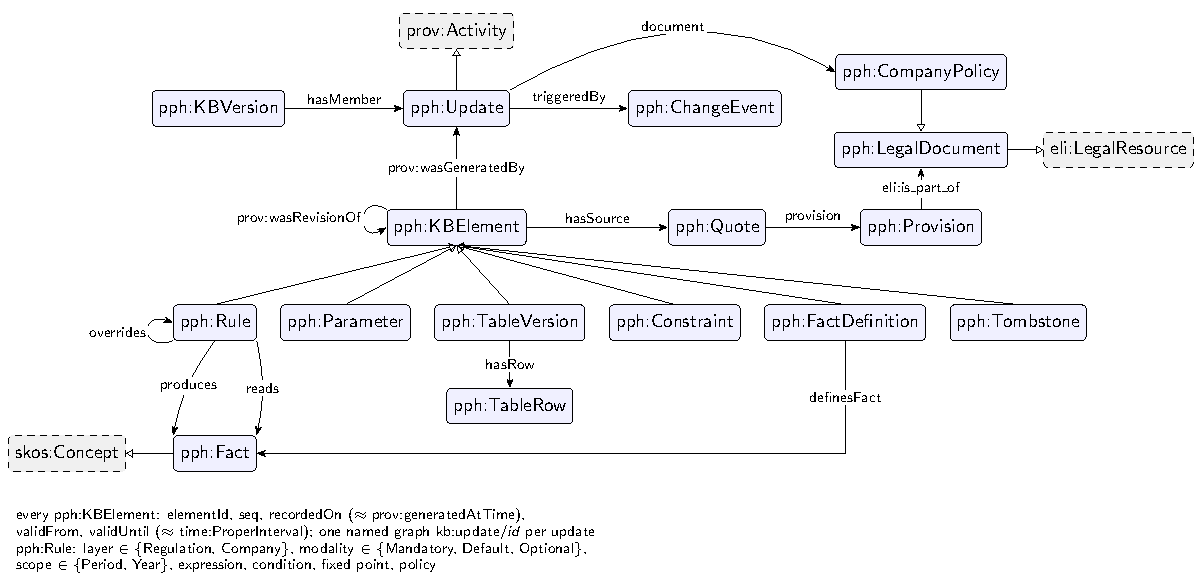
\includegraphics[width=0.72\textwidth]{ontologi.pdf}
\caption{Ontologi \en{knowledge base}. Kelas utama adalah dokumen hukum, pasal, kutipan, unsur KB (aturan, parameter, versi tabel, batasan, nisan, definisi fakta), konsep fakta, kebijakan perusahaan, peristiwa perubahan, pembaruan, dan versi KB.}
\label{fig:ontologi}
\end{figure*}

\textbf{Bahasa ekspresi.} Ekspresi adalah subset ekspresi Python satu baris dengan 27 fungsi terdaftar, misalnya \texttt{round(x, satuan, mode)}, \texttt{param}, \texttt{lookup}, \texttt{bracket}, \texttt{progressive}, \texttt{in\_table}, dan agregat masa seperti \texttt{sum\_periods} dan \texttt{cumulative}. Konstruksi lain ditolak saat \en{parse}. Tipe dasarnya \en{money} (rupiah bulat), \en{exact}, \en{rate}, \en{int}, \en{bool}, \en{category}, dan \en{date}. Semua aritmetika eksak, dan pembulatan hanya terjadi lewat \texttt{round} dengan mode dari parameter berversi, sehingga perubahan pembulatan seperti PER-11/PJ/2025 adalah pembaruan data. Kandidat LLM yang memakai fungsi atau fakta di luar kosakata tertolak di G1 atau G3.

\textbf{Semantik temporal.} Ada dua sumbu waktu. Waktu berlaku $[t_s, t_e]$ dibandingkan dengan tanggal evaluasi, yaitu tanggal 1 masa untuk aturan lingkup masa atau irisan dengan rentang kerja setahun untuk aturan lingkup tahun. Waktu pengetahuan $t_c$ adalah tanggal terbit dokumen. Pertanyaan pada $\omega$ hanya melihat rekaman dengan $t_c \leq \omega$, sehingga $\K$ bitemporal. Untuk regulasi berlaku surut ($t_s < t_c$), pertanyaan dengan $\omega \geq t_c$ menghasilkan \emph{nilai seharusnya}. Mekanisme penyelesaiannya, misalnya pembayaran tunai DTP Januari pada penggajian berikutnya, dicatat di jejak tetapi tidak dinilai, karena bergantung pada apa yang benar-benar dipotong pada tanggal penggajian.

\textbf{Batas ekspresivitas.} Representasi sengaja tidak menyatakan hubungan antar-pemberi kerja, perhitungan lintas tahun, satuan masa selain bulan, persamaan simultan, kewajiban prosedural, dan kurs valas. Penambahan fungsi adalah perubahan \en{engine}, sedangkan penambahan fakta, parameter, tabel, atau atribut kasus tidak.

\subsection{Resolusi konflik antarlapis}
Bila lebih dari satu aturan aktif untuk fakta yang sama pada konteks yang sama, \en{engine} memilih pemenang dengan tiga asas berurutan. \en{Lex superior} memberi peringkat 4 untuk aturan regulasi wajib, 3 untuk aturan perusahaan, 2 untuk aturan regulasi opsional yang diadopsi kebijakan, dan 1 untuk aturan regulasi \en{default}. Bila aturan perusahaan yang aktif kalah dari aturan wajib dengan nilai berbeda, \en{engine} mencatat konflik (A4). \en{Lex specialis} dinyatakan sebagai relasi eksplisit \texttt{overrides} antaraturan, bukan diturunkan dari sintaks kondisi, dan relasi ini harus asiklik. \en{Lex posterior} memenangkan aturan dengan $t_s$ paling akhir, lalu tanggal pencatatan rekaman pertama paling akhir, agar revisi metadata aturan lama tidak membuatnya menang kembali. Bila masih tersisa beberapa aturan dengan nilai berbeda, fakta itu tidak terdefinisi dan \en{engine} melaporkan \texttt{UnresolvedConflict}. Hierarki peraturan tidak dipakai \en{engine}; pertentangan antartingkat dinyatakan dengan \texttt{overrides}. Batasan wajib, misalnya THR paling sedikit satu bulan upah, dievaluasi setelah semua fakta dihitung, dan pelanggarannya dilaporkan dengan kode konflik.

\subsection{\en{Inference engine}}
\en{Engine} menghitung satu kasus untuk seluruh tahun pajak (Algoritma~\ref{alg:inferensi}). Evaluasi berbasis permintaan dengan memo setara dengan menelusuri graf dependensi fakta secara topologis. Aturan \en{gross-up} bertanda titik tetap dihitung dengan iterasi dari batas bawah sampai konvergen ke titik tetap terkecil. Jejak setiap fakta memuat aturan pemenang, aturan yang kalah beserta alasannya, sumber hukum, fakta yang dibaca, serta parameter dan versi tabel yang dipakai.

\begin{algorithm}[t]
\caption{Inferensi untuk satu pegawai dan satu tahun pajak}
\label{alg:inferensi}
\begin{algorithmic}[1]
\Require $\K$, kasus $x$, tanggal pengetahuan $\omega$
\State $R_\omega \gets$ rekaman terakhir per $\mathit{id}$ dengan $t_c \leq \omega$, tanpa nisan; pasang lapisan $P(x)$
\State verifikasi statis $R_\omega$ (sekali per versi)
\For{setiap fakta keluaran $f$ dan konteks $c$ (masa atau tahun)}
  \State $\mathit{kandidat} \gets$ aturan untuk $f$ yang berlaku pada tanggal evaluasi $c$
  \State $\mathit{aktif} \gets$ kandidat dengan kondisi $\varphi$ benar
  \State $r^{*} \gets$ resolusi(\en{lex superior}, \en{specialis}, \en{posterior}); catat konflik
  \State $v \gets e_{r^{*}}(c)$, atau titik tetap terkecil bila $r^{*}$ bertanda titik tetap
  \State periksa tipe; simpan memo dan jejak
\EndFor
\State evaluasi batasan wajib; catat pelanggaran
\State \Return nilai, laporan konflik, jejak
\end{algorithmic}
\end{algorithm}

% ============================================================================
\section{Akuisisi pengetahuan inkremental berbantuan LLM}
\label{sec:akuisisi}
% ============================================================================
\subsection{Pembaruan dan adaptivitas}
\label{subsec:adaptif}

\begin{definisi}[Peristiwa perubahan]
\label{def:peristiwa}
$\epsilon = \langle d, t_{\mathit{terbit}}, t_{\mathit{berlaku}}, \tau \rangle$ terdiri atas dokumen sumber, tanggal terbit (tanggal diundangkan bila ada), tanggal mulai berlaku hukum, dan jenis perubahan. Peristiwa berlaku surut bila $t_{\mathit{berlaku}} < t_{\mathit{terbit}}$. Rangkaian $\epsilon_1, \dots, \epsilon_N$, termasuk pengecoh, diurutkan menurut $t_{\mathit{terbit}}$.
\end{definisi}

\begin{definisi}[Pembaruan]
\label{def:pembaruan}
$\Delta = \langle \Delta^{+}, \Delta^{\sim}, \Delta^{-} \rangle$ berisi unsur yang ditambah, diubah, dan dicabut, dengan $\K' = \K \oplus \Delta$. Penerapan ketat menolak \en{add} untuk $\mathit{id}$ yang sudah ada dan \en{change} untuk $\mathit{id}$ yang belum ada. Pembaruan emas memenuhi $\K^{\emas}_n = \K^{\emas}_{n-1} \oplus \Delta^{\emas}_n$. $\Delta$ kosong adalah jawaban benar untuk pengecoh.
\end{definisi}

\begin{definisi}[Syarat adaptif]
\label{def:syarat}
Untuk $\K' = \K \oplus \Delta$ dan himpunan kasus $S$:
(A1) Invariansi kode. Kode \en{engine} tidak berubah.
(A2) Kesesuaian. $\hasil(\K', x, t, \omega) = \hasil(\K^{\emas}, x, t, \omega)$ untuk $x \in S$, $t \geq t_{\mathit{berlaku}}$, dan $\omega \geq t_{\mathit{terbit}}$.
(A3$_t$) Isolasi masa. Hasil untuk $t < t_{\mathit{berlaku}}$ tidak berubah, untuk semua $\omega$.
(A3$_\omega$) Isolasi pengetahuan. Hasil untuk $\omega < t_{\mathit{terbit}}$ tidak berubah.
(A4) Konsistensi lintas lapis. Laporan konflik $\K'$ sama dengan laporan konflik $\K^{\emas}$ untuk kasus yang memuat kebijakan.
\end{definisi}

\begin{definisi}[Adaptivitas representasional]
\label{def:adapt-rep}
Representasi adaptif terhadap $\epsilon$ bila \emph{ada} $\Delta$ dalam bahasa representasi yang memenuhi A1--A4. Ini sifat representasi, dibuktikan dengan menyusun $\Delta^{\emas}$ (RQ1).
\end{definisi}

\begin{definisi}[Adaptivitas operasional]
\label{def:adapt-op}
Sistem adaptif secara operasional terhadap $\epsilon$ bila pembaruan $\hat{\Delta}$ yang \emph{dipilih alur akuisisi} memenuhi A2, A3$_t$, dan A4 pada seluruh $\SE$. Satu observasi salah sudah membuat $\hat{\Delta}$ salah. Ini sifat alur akuisisi, diukur sebagai laju atas peristiwa (RQ2, RQ3).
\end{definisi}

A1 berlaku karena arsitekturnya, sebab LLM hanya menyunting \en{knowledge base}. A3$_\omega$ berlaku karena konstruksi, sebab G2 mewajibkan setiap rekaman dicatat dengan $t_c = t_{\mathit{terbit}}$. Keduanya diperiksa sebagai invarian. A1 diperiksa dengan sidik jari SHA-256 paket \en{engine}, bahasa ekspresi, dan semantik rekaman terhadap manifes yang dibekukan. Syarat yang bergantung pada LLM, yaitu A2, A3$_t$, dan A4, yang diuji.

\subsection{Alur akuisisi}
Gambar~\ref{fig:alur} menunjukkan alurnya. Teks dokumen dikunci dengan SHA-256 dan dipotong per pasal. Tabel lampiran, misalnya tarif TER, diekstraksi sekali oleh alat deterministik dan dirujuk LLM dengan id tanpa menyalin baris. Segmen dipilih dengan skor leksikal sampai 14.000 token. LLM menilai relevansi dengan kutipan, tanggal berlaku, dan subjek. Untuk dokumen relevan, konteks KB disusun lewat SPARQL, lalu LLM menyusun $m$ kandidat independen dengan kutipan per unsur. Kandidat yang lolos G1--G5, dengan satu putaran perbaikan, dikelompokkan menurut nilai fakta keluaran dan laporan konflik pada gabungan $\SG$. Kelompok terbesar menang, dan seri atau tidak adanya kandidat yang lolos berarti \en{abstain}.

\begin{figure}[t]
\centering
\begin{tikzpicture}[node distance=2.4mm]
\node[kotakdata, text width=3.2cm] (d) {Dokumen: segmen per pasal, tabel terekstraksi};
\node[kotakalur, below=of d, text width=3.2cm] (r) {Relevansi berkutipan};
\node[kotakalur, right=6mm of r, text width=2.4cm] (kosong) {$\Delta$ kosong (bila tidak relevan dan kutipan lolos G2)};
\node[kotakalur, below=of r, text width=3.2cm] (k) {Konteks KB lewat SPARQL};
\node[kotakalur, below=of k, text width=3.2cm] (m) {$m$ kandidat $\Delta$ dengan kutipan};
\node[kotakalur, below=of m, text width=3.2cm] (g) {G1 struktur, G2 kutipan, G3 statis, G4 regresi, G5 non-vakuitas};
\node[kotakalur, right=6mm of g, text width=2.4cm] (p) {Satu putaran perbaikan dengan pesan gerbang};
\node[kotakalur, below=of g, text width=3.2cm] (c) {Konsensus perilaku pada $\SG$};
\node[kotakalur, right=6mm of c, text width=2.4cm] (a) {\en{Abstain}: seri atau tidak ada yang lolos};
\node[kotakdata, below=of c, text width=3.2cm] (kb) {Peninjau dengan laporan dampak, lalu $\K'$};
\draw[panah] (d) -- (r);
\draw[panah] (r) -- (kosong);
\draw[panah] (r) -- (k);
\draw[panah] (k) -- (m);
\draw[panah] (m) -- (g);
\draw[panah] (g.east) -- (p.west);
\draw[panah] (p.north) |- (m.east);
\draw[panah] (g) -- (c);
\draw[panah] (c) -- (a);
\draw[panah] (c) -- (kb);
\end{tikzpicture}
\caption{Alur akuisisi pengetahuan inkremental. Dalam operasi, peninjau memeriksa pembaruan dengan laporan dampak sebelum versi baru berlaku.}
\label{fig:alur}
\end{figure}

\subsection{Gerbang verifikasi}
Tabel~\ref{tab:gerbang} merangkum gerbang. Untuk G4 dan G5, setiap unsur $u$ diberi \emph{tanggal mulai efek} $s(u)$, yaitu tanggal pertama di mana rekaman yang berlaku untuk $\mathit{id}$-nya dapat berbeda antara $\K$ dan $\K'$. Dengan begitu, pembaruan yang menutup masa berlaku aturan lama tidak keliru dianggap regresi.

\begin{table}[t]
\centering
\caption{Gerbang verifikasi dan syarat yang dijaganya}
\label{tab:gerbang}
\scriptsize
\begin{tabularx}{\columnwidth}{@{}P{0.5cm} L P{1.3cm}@{}}
\toprule
\textbf{ID} & \textbf{Pemeriksaan} & \textbf{Syarat} \\
\midrule
G1 & Skema keluaran, penerapan ketat, dan 15 \en{shape} inti serta 12 batasan SHACL-SPARQL atas $\K'$ & validitas \\
G2 & Kutipan $\geq$ 20 karakter adalah \en{substring} teks yang dinormalisasi; setiap bilangan $\geq 100$, pecahan, dan tanggal baru muncul di kutipan unsurnya; $t_c = t_{\mathit{terbit}}$ & keberadaan kutipan, A3$_\omega$ \\
G3 & Verifikasi statis ekspresi, graf dependensi asiklik kecuali titik tetap, tanpa rujukan menggantung; peringatan anomali & A4 \\
G4 & Regresi pada $\SG$: hasil sebelum $s(\Delta)$ dan hasil dengan $\omega < t_{\mathit{terbit}}$ tidak berubah; tanpa galat \en{engine} baru & A3$_t$ \\
G5 & Non-vakuitas untuk $\Delta$ tidak kosong: setiap unsur yang ditambah atau diubah mengubah minimal satu fakta keluaran atau laporan konflik pada $\SG$ sesudah $s(u)$; unsur yang dicabut pernah menyala; tanggal dan subjek dari penilaian relevansi tercermin & menolak pembaruan tanpa efek \\
\bottomrule
\end{tabularx}
\end{table}

Tanpa G5, pembaruan kosong atau aturan yang tidak pernah menyala lolos semua gerbang, karena keduanya tidak menimbulkan regresi. Pembaruan kosong hanya dapat diterapkan lewat penilaian relevansi berkutipan, sehingga G5 tidak bertentangan dengan pengecoh.

$\SG$ dibangkitkan per kandidat dari $\K \oplus \hat{\Delta}$ tanpa membaca emas atau $\SE$. Generator menyasar bulan sekitar $s(u)$, ambang pada $b-1$, $b$, dan $b+1$, atribut kasus di kondisi, pola kerja, serta komponen tidak teratur dan natura, paling banyak 300 kasus. Komponen penanda senilai 7 rupiah menjamin $\SG \cap \SE = \varnothing$. Syarat pembekuan gerbang adalah laju penolakan keliru nol atas $\Delta^{\emas}$ pengembangan. Dalam praktik, gerbang juga disesuaikan sampai $\Delta^{\emas}$ peristiwa uji lolos (Bagian~\ref{subsec:ancaman}).

\subsection{Analisis dampak lintas lapis}
Kebijakan $P$ \emph{terdampak} oleh peristiwa $\epsilon_n$ bila, pada kasus $\SE$ yang memuat $P$, (a) nilai fakta yang dihasilkan aturan $P$ berubah untuk minimal satu observasi sesudah $t_{\mathit{berlaku}}$, (b) aturan pemenang suatu fakta yang dihasilkan atau dibaca $P$ berubah, atau (c) muncul entri konflik baru yang melibatkan $P$. Label (a) dan (b) diturunkan dari eksekusi $\K^{\emas}_{n-1} \oplus P$ dan $\K^{\emas}_n \oplus P$, sedangkan detektor bekerja statis pada graf, sehingga label tidak tautologis. Detektor menghitung $F_\Delta$, yaitu fakta yang dihasilkan unsur $\Delta$ dan fakta yang dihasilkan aturan pemakai parameter atau tabel di $\Delta$, lalu penutup hilirnya lewat \texttt{pph:reads}. Aturan $P$ yang membaca fakta di penutup itu dengan masa berlaku beririsan ditandai (a). Aturan $P$ yang menghasilkan fakta yang sama dengan aturan $\Delta$ ditandai (b), dan (c) bila aturan $\Delta$ itu wajib. Kuerinya ditulis dalam SPARQL dan dibekukan sebelum E4.

\subsection{Konfigurasi LLM}
Model utama adalah Claude Opus 5.5 dengan \en{training cutoff} Juni 2026 (pengenal API \texttt{claude-opus-5-5}), dipakai dengan \en{effort} \texttt{medium} untuk relevansi dan \texttt{high} untuk penyusunan dan perbaikan. Model kedua adalah \texttt{gpt-6.1-sol} (\en{cutoff} 30 April 2026) dengan \en{reasoning effort} \texttt{high}. Parameter \en{sampling} tidak dapat diatur pada kedua model, sehingga keragaman kandidat berasal dari \en{sampling} bawaan. Keluaran memakai \en{structured output} dengan skema datar, dan awalan bersama disimpan dengan \en{prompt caching}. Panggilan eksperimen dijalankan pada 28--29 Oktober 2026 dan dicatat lengkap, yaitu \en{prompt}, keluaran mentah, token, biaya, durasi, dan hasil setiap gerbang, sehingga semua analisis dapat diulang tanpa memanggil LLM lagi.

% ============================================================================
\section{Metodologi evaluasi}
\label{sec:evaluasi}
% ============================================================================
Setiap RQ punya satu metrik utama yang ditetapkan sebelum eksperimen. Kebenaran diukur dari perilaku hasil perhitungan, data sistem terpisah dari data penilai, alat ukur divalidasi lebih dulu, dan hasil dilaporkan sebagai estimasi dengan selang kepercayaan eksak.

\subsection{Desain penelitian dan pra-registrasi}
Penelitian ini mengikuti \en{design science research}. Hipotesis, metrik utama, ambang, pembagian data, kasus uji, dan rencana analisis dikunci dengan \en{tag} git \texttt{prareg} sebelum peristiwa uji pertama dijalankan. Alur akuisisi, \en{prompt}, gerbang, generator $\SG$, dan aturan konsensus dibekukan dengan \en{tag} \texttt{alur-beku}, \en{engine} dengan \texttt{engine-v1}, dan emas dengan \texttt{emas-v1}. Analisis terdiri atas tiga jenis. Pemeriksaan invarian mencakup A1 dan A3$_\omega$. Analisis konfirmatori menguji hipotesis dengan metrik utama. Analisis eksploratori memakai metrik diagnostik.

Anggaran awal LLM adalah USD 15 untuk seluruh penelitian. Anggaran itu habis sesudah strata utama E2 dan E3. E4 tidak memakai LLM, karena masukannya $\Delta^{\emas}$. Sesudah hasil awal terlihat, peneliti menambah anggaran dan menulis amandemen 1 (\en{tag} \texttt{prareg-amandemen-1}) sebelum jalan tambahan mana pun. Amandemen tidak mengubah alur, \en{engine}, emas, $\SE$, ambang, atau $\delta_S$. Karena hasil awal sudah terlihat, amandemen ini \emph{tidak buta}. Jalan yang ditambahkan lewat amandemen adalah sembilan pengecoh sisa sehingga H3a diuji pada $N = 33$ sesuai rancangan, jalan terisolasi kedua untuk batas derau H3b, rantai pembangkitan ulang untuk komponen kontekstual H3b, sensitivitas $m = 5$, model kedua, strata kontrafaktual dan kebijakan buatan, ablasi AB1, AB2, dan AB5, pembanding B2, analisis kontaminasi, dan label ketepatan kutipan. Kecuali tiga yang pertama, semuanya berstatus eksploratori. Detektor dampak v2 dan penyelarasan kunci konflik pada penilai A4 juga dibuat sesudah hasil awal terlihat.

\subsection{Pembagian data dan kronologi}
\label{subsec:pembagian}
\begin{itemize}[leftmargin=*,nosep]
  \item \textbf{Pengembangan.} 13 peristiwa yang terbit 2012--2022 dan berlaku 2013--2022 (D01--D13), lima regulasi fiktif (FR01--FR05), dan PKB TPK Koja 2012. Data ini dipakai untuk merancang \en{prompt}, gerbang, dan aturan pemilihan, lalu ketiganya dibekukan.
  \item \textbf{Uji.} 13 peristiwa nyata 2023--2026 (E01--E13), 20 pengecoh, lima PKB nyata, 14 kebijakan buatan, empat dokumen kontrafaktual, dan 16 perubahan tak terlihat. Peristiwa uji tidak pernah dijalankan alur sebelum \en{tag} \texttt{prareg}, diperiksa dari log panggilan. Representasi, \en{engine}, dan $\K^{\emas}$ disusun dengan mengetahui peristiwa ini, dan akibatnya ditangani di Bagian~\ref{subsec:hindsight}.
  \item \textbf{Uji prospektif.} Regulasi yang terbit sesudah \en{tag} \texttt{prareg} dipantau. Sampai naskah ini ditulis belum ada peristiwa prospektif yang relevan.
\end{itemize}

\subsection{Bias pandangan belakang}
\label{subsec:hindsight}
Representasi dan \en{engine} dikembangkan ketika semua perubahan dalam rentang uji sudah terbit, sehingga klaim \emph{tanpa mengubah kode} untuk peristiwa itu lemah. Ada dua mitigasi. Pertama, riwayat \en{engine} dipublikasikan, dan 16 kemampuan \en{engine} dipetakan ke regulasi yang membutuhkannya. Kedua, 16 perubahan struktural sintetis (U01--U16) ditulis oleh agen terpisah yang hanya membaca taksonomi perubahan dan dataset regulasi, lalu disegel dengan manifes \en{hash} sebelum representasi dibekukan. Setiap perubahan disertai teks dan contoh hitungan, seluruhnya 100 contoh. Perubahan itu dihitung berhasil (RA $=1$) hanya bila $\Delta$ yang disusun mereproduksi seluruh contoh tanpa mengubah \en{engine}. $\Delta$ disusun dan diuji oleh agen pelaksana lain yang tidak ikut merancang representasi, dan hasilnya diperiksa ulang oleh agen peninjau ketiga. Perancang hanya menerima hasil. Pemeriksaan manusia atas perubahan dan $\Delta$-nya sesudah segel dibuka belum dilakukan.

\subsection{Rantai kepercayaan dan validasi instrumen}
\label{subsec:instrumen}
Semua angka RQ2--RQ4 bergantung pada $\K^{\emas}$ dan $\SE$, sehingga keduanya divalidasi lebih dulu sebagai instrumen (E0). Gambar~\ref{fig:rantai} menunjukkan rantainya.

\begin{figure}[t]
\centering
\begin{tikzpicture}[node distance=2.5mm]
\node[kotakdata, text width=1.45cm, minimum height=1.05cm] (g1) {GT1 contoh resmi (\en{holdout})};
\node[kotakdata, right=1.5mm of g1, text width=1.45cm, minimum height=1.05cm] (g2) {GT2 kalkulator DJP};
\node[kotakdata, right=1.5mm of g2, text width=1.45cm, minimum height=1.05cm] (g3) {GT3 50 kasus bertingkat};
\node[kotakdata, right=1.5mm of g3, text width=1.45cm, minimum height=1.05cm] (g5) {GT5 contoh kebijakan};
\node[kotakalur, below=6mm of $(g2.south)!0.5!(g3.south)$, text width=6.3cm] (kemas) {$\K^{\emas}_n$ dan $\Delta^{\emas}_n$ (emas sebagai kode, kutipan terverifikasi otomatis, pembaca kedua)};
\node[kotakalur, below=of kemas, text width=6.3cm] (se) {Nilai harapan $\SE$ (2.398 kasus); kecukupan diukur dengan \en{mutation score}};
\node[kotakalur, below=of se, text width=3.3cm] (dh) {Penilaian $\hat{\Delta}$: A2, A3$_t$, A4};
\node[kotakdata, left=2mm of dh, text width=1.5cm] (sg) {$\SG$ hanya untuk gerbang};
\foreach \g in {g1,g2,g3,g5} \draw[panah] (\g.south) -- (\g.south |- kemas.north);
\draw[panah] (kemas) -- (se);
\draw[panah] (se) -- (dh);
\draw[dashed] (sg.north) -- node[label, left]{$\SG \cap \SE = \varnothing$} ++(0,0.55);
\end{tikzpicture}
\caption{Rantai kepercayaan \en{ground truth}. Acuan memvalidasi emas, emas menghasilkan nilai harapan $\SE$, dan $\SE$ menilai pembaruan dari LLM.}
\label{fig:rantai}
\end{figure}

\begin{enumerate}[leftmargin=*,nosep]
  \item \textbf{Acuan.} GT1 adalah contoh perhitungan resmi di lampiran regulasi, dibagi menjadi bagian pengembangan dan 14 berkas \en{holdout} yang hanya dibuka sekali. GT2 adalah kalkulator PPh 21 resmi DJP, dengan 20 kasus bulanan dan 15 kasus masa pajak terakhir. GT3 adalah 50 kasus bertingkat 2023--2026 yang dihitung langkah demi langkah dari teks regulasi dengan penghitung terpisah dari \en{engine}. GT5 adalah 21 contoh hitungan dari klausul lima PKB nyata. Implementasi pihak ketiga (GT4) dikumpulkan, tetapi tidak masuk validasi yang dilaporkan di sini.
  \item \textbf{Adjudikasi selisih.} Setiap selisih diputuskan sebagai kesalahan KB, kesalahan acuan, atau ambiguitas hukum. Titik yang regulasinya diam atau ambigu diputuskan dalam 18 tafsir perhitungan (K1--K18) dan tafsir semantik berlaku surut.
  \item \textbf{Uji \en{engine}.} \en{Engine} diuji terpisah dengan uji unit atas aritmetika, 12 uji resolusi konflik dengan pemenang hukum yang diketahui, uji mutasi SHACL dan G3, serta pemeriksaan kesetaraan dengan \en{engine} prototipe.
  \item \textbf{Kecukupan $\SE$.} \en{Mutation score} terfokus-$\Delta$ per peristiwa dihitung atas mutan yang tidak setara, dengan ambang 0,80. Peristiwa di bawah ambang ditambah kasus terarah.
  \item \textbf{Keandalan $\Delta^{\emas}$.} Dua agen peninjau independen tanpa konteks penyusun mengodekan ulang $\Delta^{\emas}$ regulasi E01--E13 dan kebijakan buatan dari teks dokumen dan basis KB, lalu membandingkannya dengan emas. Pengodean ini buta terhadap emas, tetapi tidak terhadap basis KB yang sama dengan konteks LLM. Lima PKB nyata hanya diperiksa terhadap emas, tanpa pengodean ulang buta. Kesepakatan dilaporkan dengan Krippendorff's $\alpha$.
  \item \textbf{Syarat lulus E0.} Tidak ada selisih berstatus \emph{KB salah} yang belum diselesaikan pada tahun uji, dan \en{mutation score} mencapai ambang.
  \item \textbf{Protokol koreksi emas.} Bila keluaran LLM atau peninjauan menyingkap kesalahan emas, emas diperbaiki dengan \en{commit} bertanda, $\SE$ dibangun ulang, semua kondisi dan semua jalan dinilai ulang, dan jumlah koreksi dilaporkan. Koreksi tidak boleh dibuat hanya pada peristiwa tempat usulan kalah.
\end{enumerate}

\subsection{Ruang uji}
\label{subsec:ruanguji}
$\SE$ berisi 2.398 kasus pegawai-tahun dari tiga kriteria (Tabel~\ref{tab:cakupan}). Cakupan kombinatorial berbatasan mencakup seluruh kombinasi 2-arah yang sah menurut batasan antardimensi. Cakupan batas menguji setiap batas lapisan TER dan Pasal 17 di $b-1$, $b$, dan $b+1$. Kasus batas Pasal 17 dibangkitkan terbalik dari PKP ke bruto. Sampel operasional diambil acak dari sel upah provinsi dan lapangan usaha BPS. Kasus kebijakan berjumlah 120--180 per kebijakan untuk 19 kebijakan, dan 21 kasus terarah ditambahkan dari analisis mutan dan koreksi emas.

\begin{table}[t]
\centering
\caption{Ruang uji $\SE$ dan cakupannya}
\label{tab:cakupan}
\scriptsize
\begin{tabularx}{\columnwidth}{@{}L P{1.6cm} P{2.0cm}@{}}
\toprule
\textbf{Kriteria} & \textbf{Kasus per tahun} & \textbf{Cakupan} \\
\midrule
Batas lapisan Pasal 17 & 15 & 2023--2026 \\
Batas lapisan TER (A, B, C) & 321 & 2024--2026 \\
Kombinasi 2-arah berbatasan & 42--45 & 100\% \\
Kombinasi 3-arah berbatasan & (kasus yang sama) & 62--64\% \\
Sampel operasional acak (BPS) & 300 & 2023--2026 \\
\midrule
Jumlah kasus regulasi & \multicolumn{2}{l}{2.398} \\
Kasus kebijakan & \multicolumn{2}{l}{19 kebijakan $\times$ 120--180} \\
\bottomrule
\end{tabularx}
\end{table}

\subsection{Korpus}
\label{subsec:korpus}

\subsubsection{Peristiwa perubahan nyata}
Tabel~\ref{tab:korpus} memuat ke-13 peristiwa uji, termasuk empat surat batas upah Jaminan Pensiun tahunan, karena iuran pensiun pegawai adalah pengurang PPh 21. Satu dokumen semula digolongkan pengecoh administrasi, yaitu PER-11/PJ/2025. Saat spesifikasi disusun ternyata dokumen itu mengubah pembulatan PPh 21 sejak Masa Januari 2025, sehingga dipindah menjadi peristiwa uji E13. Rantai emas utama berisi 37 pembaruan dengan 282 rekaman, ditambah 27 pembaruan sisi untuk regulasi fiktif dan kebijakan.

\begin{table}[t]
\centering
\caption{Korpus peristiwa perubahan dan hasil E2 usulan (B benar, S salah, A \en{abstain}). Pada kebijakan buatan, dua dari lima B tidak teruji pada $\SE$ dan hasil ini dicatat sesudah koreksi emas (sebelumnya 3 B, 8 S, 3 A). Baris SP dan CF dijalankan lewat amandemen 1}
\label{tab:korpus}
\scriptsize
\setlength{\tabcolsep}{3pt}
\begin{tabularx}{\columnwidth}{@{}P{0.55cm} L P{1.0cm} P{1.1cm} P{0.55cm} P{0.75cm}@{}}
\toprule
\textbf{No.} & \textbf{Dokumen} & \textbf{Berlaku} & \textbf{Jenis} & $|\Delta^{\emas}|$ & \textbf{E2} \\
\midrule
E01 & Surat BPJS TK, batas upah JP 2023 & 2023-03 & T1 & 1 & B \\
E02 & PMK 66/2023 (natura) & 2023-07 & T3 & 15 & S \\
E03 & PP 58/2023 (TER) & 2024-01 & T2, T7; S4, S6 & 7 & B \\
E04 & PMK 168/2023 (juklak TER) & 2024-01 & T7, T3; S4 & 14 & A \\
E05 & Surat BPJS TK, batas upah JP 2024 & 2024-03 & T1 & 1 & B \\
E06 & PMK 10/2025 (DTP padat karya) & 2025-01 & T4; S1--S3 & 15 & A \\
E07 & PP 7/2025 (keringanan JKK) & 2025-02 & T1; S1--S3 & 2 & S \\
E08 & Surat BPJS TK, batas upah JP 2025 & 2025-03 & T1 & 1 & B \\
E13 & PER-11/PJ/2025 (pembulatan) & 2025-01 & T9; S1 & 1 & B \\
E09 & PP 36/2025 (perpanjangan JKK) & 2025-08 & T6; S1--S3, S5 & 2 & B \\
E10 & PMK 72/2025 (DTP pariwisata) & 2025-10 & T5; S1--S3, S5 & 5 & B \\
E11 & PMK 105/2025 (DTP 2026) & 2026-01 & T4; S2, S3 & 11 & S \\
E12 & Surat BPJS TK, batas upah JP 2026 & 2026-03 & T1 & 1 & B \\
\midrule
P01--P21 & 20 pengecoh (X1--X5) & -- & tidak relevan & 0 & 1 S \\
PKB & 5 PKB nyata (WIKA, Centex, AVCO, Taekwang, Sansan) & -- & T10 & 14--35 & 5 A \\
SP & 14 kebijakan buatan & -- & T10 & 1--7 & 5 B, 6 S, 3 A \\
CF & 4 kontrafaktual (dari E01, E02, E06, E11) & -- & T1, T3, T4 & -- & 1 B, 1 S, 2 A \\
U & 16 perubahan tak terlihat & -- & T1--T10 & -- & -- \\
D, FR & 13 pengembangan, 5 fiktif & 2013--2022 & T1--T9 & 0--20 & -- \\
\bottomrule
\end{tabularx}
\end{table}

\subsubsection{Dokumen pengecoh}
Ke-20 pengecoh menyebut PPh 21 atau iuran tetapi tidak mengubah perhitungan pegawai tetap, misalnya ketentuan Coretax, DTP peserta magang, dan rekomposisi iuran JKK untuk JKP (P01). Jawaban benarnya pembaruan kosong.

\subsubsection{Dokumen kontrafaktual}
Empat dokumen kontrafaktual mengubah nilai atau ambang dokumen nyata secara konsisten, dengan $\Delta^{\emas}$ yang diturunkan terprogram. Varian ini bukan sampel independen.

\subsubsection{Perubahan tak terlihat}
Ke-16 perubahan mencakup jenis T1--T10, misalnya kategori TER keempat (U03), iuran Tapera sebagai pengurang (U04), fasilitas DTP dengan syarat usia (U06), dasar TER dibulatkan ke ribuan (U11), dan dua perubahan lapisan perusahaan (U14, U15). Semua bertanggal sesudah 25 Februari 2026, sehingga basisnya rantai emas lengkap.

\subsubsection{Kebijakan perusahaan}
Lima PKB nyata yang terbuka untuk umum menjadi strata kebijakan uji. Empat belas kebijakan buatan, termasuk tiga kontrol negatif, melengkapi jenis konflik yang tidak muncul di PKB nyata, dan dilaporkan terpisah. Setiap dokumen kebijakan juga menjadi masukan E2, dengan $\Delta^{\emas}$ yang disusun seperti dokumen regulasi. Pemeriksaannya berbeda: kebijakan buatan dikodekan ulang secara buta oleh pembaca kedua, sedangkan lima PKB nyata hanya diperiksa terhadap emas.

\subsection{Mode evaluasi dan hasil per dokumen}
\begin{itemize}[leftmargin=*,nosep]
  \item \textbf{Mode terisolasi (RQ2).} $\hat{\Delta}_n$ diterapkan pada $\K^{\emas}_{n-1}$ dan dinilai pada $\SE_n$.
  \item \textbf{Mode berantai (RQ3).} $\hat{\Delta}_n$ diterapkan pada $\K^{\mathrm{sis}}_{n-1}$, yaitu hasil pembaruan sistem sendiri. Rantai dimulai dari $\K^{\emas}_0$ (rekaman sampai 2022) dan memakai 150 kasus $\SE$ per tahun. Ada dua cara memperoleh $\hat{\Delta}_n$. Pada rantai \emph{transplantasi}, $\hat{\Delta}_n$ adalah hasil E2 terisolasi yang dipindah ke $\K^{\mathrm{sis}}_{n-1}$, dengan penerapan longgar bila perlu. Pada rantai \emph{pembangkitan ulang}, yang dijalankan lewat amandemen 1, $\hat{\Delta}_n$ dibangkitkan dengan $\K^{\mathrm{sis}}_{n-1}$ sebagai konteks, sesuai Definisi~\ref{def:adapt-op} sepenuhnya. Kesalahan dihitung per kasus pegawai-tahun.
  \item Kedua mode berjalan tanpa peninjau, sehingga hasilnya batas bawah kinerja. Setiap dokumen relevan berakhir sebagai benar-diterapkan, salah-diterapkan (kesalahan senyap), atau \en{abstain}; dokumen relevan yang dinilai tidak relevan dihitung salah. Pengecoh tidak masuk SER dan CAR.
  \item \textbf{\en{Abstain} pada mode berantai.} Varian \emph{tetap} mempertahankan KB lama; varian \emph{peninjau sempurna} menyisipkan $\Delta^{\emas}_n$. Analisis konfirmatori memakai jalan pertama per dokumen nyata.
\end{itemize}

\subsection{Pembanding dan ablasi}
Tabel~\ref{tab:pembanding} merangkum kondisi pembanding. B3, B4, AB3, dan AB4 dihitung dari kandidat dan log gerbang yang sama dengan usulan, tanpa panggilan LLM baru. B4 memakai $m$ kandidat awal, lebih sedikit daripada usulan yang juga memakai putaran perbaikan.

\begin{table}[t]
\centering
\caption{Pembanding dan ablasi}
\label{tab:pembanding}
\scriptsize
\begin{tabularx}{\columnwidth}{@{}P{0.6cm} L P{0.95cm}@{}}
\toprule
\textbf{ID} & \textbf{Kondisi} & \textbf{RQ} \\
\midrule
\multicolumn{3}{@{}l}{\textit{Pembanding}} \\
B1 & Praktik saat ini: riwayat \en{commit} kalkulator PPh 21 sumber terbuka di sekitar pergantian ke TER & motivasi \\
B2 & LLM menghitung PPh 21 langsung dari 26 dokumen yang berlaku pada 100 kasus operasional 2025 & motivasi \\
B3 & Kandidat pertama yang lolos G1--G2, tanpa perbaikan (\en{pass@1}) & RQ2 \\
B4 & Suara terbanyak menurut perilaku atas $m$ kandidat awal, tanpa gerbang & RQ2 \\
B5 & Analisis dampak: (i) tandai semua kebijakan yang menyentuh fakta di penutup hilir $F_\Delta$; (ii) pemindaian teks ekspresi tanpa graf & RQ4 \\
\midrule
\multicolumn{3}{@{}l}{\textit{Ablasi (model utama)}} \\
AB1 & Formalisasi dari nol pada keadaan hukum 2023 dan 2024: basis hanya kosakata fakta, masukan seluruh dokumen yang berlaku & RQ2, RQ3 \\
AB2 & Tanpa konteks \en{knowledge base} & RQ2 \\
AB3 & Tanpa G5, tanpa G4, atau tanpa putaran perbaikan & RQ2 \\
AB4 & Pemilihan pertama lolos, konsensus, atau seleksi sempurna & RQ2 \\
AB5 & Validasi skema biasa dibanding \en{shape} SHACL & RQ2 \\
\bottomrule
\end{tabularx}
\end{table}

\subsection{Hipotesis dan metrik utama}
Tabel~\ref{tab:lacak} memuat hipotesis, metrik utama, dan ambangnya. Setiap ambang ditetapkan pada atau di atas batas terbaik yang dapat dicapai jumlah sampel yang direncanakan. Contohnya, dengan 18 dokumen tanpa kesalahan, batas atas eksak SER sebesar 0,153, sehingga $\theta_2 = 0{,}25$ masih dapat dicapai dengan satu kesalahan (batas atas 0,238).

\begin{table*}[t]
\centering
\caption{Keterlacakan kontribusi, RQ, hipotesis, dan metrik utama}
\label{tab:lacak}
\scriptsize
\begin{tabularx}{\textwidth}{@{}P{1.2cm} L P{4.0cm} P{3.6cm} P{1.3cm}@{}}
\toprule
\textbf{RQ} & \textbf{Hipotesis} & \textbf{Metrik utama} & \textbf{Analisis} & \textbf{Eksperimen} \\
\midrule
-- & Invarian A1 dan A3$_\omega$ tanpa pelanggaran & jumlah pelanggaran & pemeriksaan & semua \\
RQ1 (K1) & H1: batas bawah satu sisi 95\% RA perubahan tak terlihat $\geq \theta_1 = 0{,}70$ & RA, proporsi perubahan yang dapat dinyatakan tanpa mengubah \en{engine} & Clopper--Pearson & E1 \\
RQ2 (K2) & H2a: batas atas satu sisi 95\% SER usulan $\leq \theta_2 = 0{,}25$. H2b: CAR usulan lebih tinggi daripada B3 dan B4, dan SER usulan tidak lebih buruk dengan margin $\delta_S = 0{,}10$ & SER dan CAR atas 18 dokumen nyata & Clopper--Pearson; McNemar eksak satu sisi; selisih berpasangan dengan CI Newcombe; Holm & E2 \\
RQ3 (K3) & H3a: batas bawah satu sisi 95\% OAR $\geq \theta_3 = 0{,}75$. H3b: kesalahan terpicu tidak melebihi batas derau & OAR atas 33 peristiwa; kesalahan terpicu $I$ & Clopper--Pearson; deskriptif terhadap batas derau & E3 \\
RQ4 (K1) & H4a: batas bawah CI 95\% \en{recall} $\geq \theta_4 = 0{,}70$. H4b: $F_2$ detektor lebih tinggi daripada B5(i) dan B5(ii) & \en{Recall} dan $F_2$ atas pasangan kebijakan dan peristiwa & \en{bootstrap} klaster per peristiwa; Holm & E4 \\
\bottomrule
\end{tabularx}
\end{table*}

\subsubsection{Definisi metrik utama}
\begin{itemize}[leftmargin=*,nosep]
  \item \textbf{RA (RQ1).} Proporsi perubahan yang dapat dinyatakan sebagai $\Delta$ yang mereproduksi seluruh contoh tanpa mengubah \en{engine}. Untuk peristiwa nyata dan kebijakan, RA dilaporkan sebagai bukti konstruktif $\Delta^{\emas}$ beserta kecocokannya dengan acuan. Hanya perubahan tak terlihat yang menguji H1.
  \item \textbf{SER dan CAR (RQ2).} Dihitung atas himpunan $D$ yang berisi 13 regulasi dan 5 PKB nyata, satu hasil per dokumen. $\mathrm{SER} = \frac{1}{|D|}\sum_{d} \mathbf{1}[\text{salah-diterapkan}]$, $\mathrm{CAR} = \frac{1}{|D|}\sum_{d} \mathbf{1}[\text{benar-diterapkan}]$, dan $\mathrm{ABS} = 1 - \mathrm{SER} - \mathrm{CAR}$. SER mengukur keamanan dan CAR mengukur kegunaan. Keduanya dilaporkan bersama, karena sistem yang selalu \en{abstain} punya SER nol tetapi tidak berguna. Dari keduanya diturunkan cakupan CAR $+$ SER dan risiko selektif SER$/$(CAR $+$ SER)~\cite{xin2021abstention}.
  \item \textbf{OAR (RQ3).} Proporsi peristiwa yang tidak memperkenalkan kesalahan baru dalam mode berantai. A2, A3$_t$, dan A4 dinilai pada $\SE_{\leq n}$, gabungan kasus semua keadaan sampai peristiwa $n$, di luar kasus $H_n$ yang sudah salah sebelum peristiwa itu. Satuannya adalah kasus pegawai-tahun: sebuah kasus salah bila minimal satu observasinya salah. Tanpa pengecualian $H_n$, satu kesalahan lama terhitung ulang di setiap peristiwa berikutnya.
  \item \textbf{Kesalahan terpicu (RQ3).} $I_n = E^{\mathrm{ber}}_n \setminus (E^{\mathrm{iso}}_n \cup H_n)$, yaitu kasus yang salah pada mode berantai tetapi tidak salah pada mode terisolasi dan belum salah sebelumnya. Komponen mekanis diperoleh dengan memindahkan $\hat{\Delta}_n$ terisolasi ke $\K^{\mathrm{sis}}_{n-1}$. Komponen kontekstual diperoleh dari pembangkitan ulang. Batas derau diperkirakan dari selisih dua jalan terisolasi yang independen.
  \item \textbf{\en{Recall} dan $F_2$ (RQ4).} Dihitung atas pasangan kebijakan dan peristiwa, dengan $F_2 = 5PR/(4P+R)$. \en{Recall} diutamakan karena kebijakan terdampak yang terlewat lebih berbahaya daripada peringatan palsu. Pembanding \emph{tandai semuanya} menghasilkan $F_2 = 5\pi/(4\pi+1)$ untuk prevalensi $\pi$.
\end{itemize}

\subsubsection{Metrik diagnostik}
Metrik diagnostik bersifat eksploratori: selisih terhadap acuan dan \en{mutation score} untuk instrumen; akurasi resolusi konflik dan kelengkapan jejak untuk RQ1; \en{pass@1}, \en{pass@m}, dan \en{1@m} pada kandidat sebelum perbaikan, dengan $\text{pass@}j = 1-\binom{m-c}{j}/\binom{m}{j}$ dan efisiensi pemilihan $\eta = (\text{1@}m - \text{pass@}1)/(\text{pass@}m - \text{pass@}1)$~\cite{li2022alphacode}, laju hafalan, kontaminasi, positif palsu relevansi, ketepatan kutipan, dan biaya untuk RQ2; kasus salah di akhir rangkaian untuk RQ3; presisi dan Cohen's $\kappa$ untuk RQ4.

\subsection{Analisis statistik}
\label{subsec:statistik}
Proporsi dilaporkan dengan CI eksak Clopper--Pearson. Perbandingan berpasangan antarkondisi memakai selisih risiko dengan CI Newcombe dan uji McNemar eksak satu sisi. Non-inferioritas SER diterima bila batas atas CI selisih SER berpasangan kurang dari $\delta_S$. RQ4 memakai \en{bootstrap} klaster per peristiwa. Keluarga Holm RQ2 berisi CAR terhadap B3 dan B4 serta dua uji non-inferioritas, dan keluarga RQ4 berisi selisih $F_2$ terhadap B5(i) dan B5(ii). Unit analisisnya dokumen sumber nyata untuk RQ2 dan peristiwa untuk RQ3 dan RQ4. RQ3 bersyarat pada satu rangkaian dengan $R = 1$ dan dibaca deskriptif. Simulasi daya menunjukkan bahwa dengan $N = 18$ dan $\alpha = 0{,}025$, McNemar baru mencapai daya 80\% pada selisih CAR sekitar 0,45, sehingga kegagalan menolak H2b tidak dibaca sebagai bukti kesetaraan.

\subsection{Prosedur eksperimen}
E0 memvalidasi instrumen (Bagian~\ref{subsec:instrumen}). E1 menguji perubahan tak terlihat, peristiwa nyata, dan kebijakan. E2 menjalankan 13 regulasi uji dengan $m = 3$ dan 5 PKB dengan $m = 2$, satu putaran perbaikan, dan \en{seed} 20261027; pengecoh memakai $m = 1$ bila dinilai relevan, sedangkan kontrafaktual dan kebijakan buatan $m = 2$. E3 memutar 33 peristiwa dengan dua varian \en{abstain}, dua cara memperoleh $\hat{\Delta}_n$, dan $R = 1$. E4 menilai 134 pasangan kebijakan dan peristiwa dengan masukan $\Delta^{\emas}$. E5 berisi B1 dan B2.

\subsection{Biaya dan kelayakan}
Rancangan semula dengan $m = 5$, seluruh ablasi, dan model kedua diperkirakan di atas USD 30, padahal anggaran awal USD 15, sehingga $m$ diturunkan dan E3 memakai $R = 1$. Biaya per dokumen USD 0,12--1,87 untuk regulasi, 0,47--0,90 untuk PKB, dan 0,04--0,45 untuk pengecoh. Pengeluaran akhir sekitar USD 81,6 untuk Claude dan USD 8,1 untuk OpenAI.

\subsection{Kolaborator dan rencana cadangan}
Penelitian ini dikerjakan peneliti tunggal. Peran kolaborator manusia diisi agen AI independen yang tidak membawa konteks penyusunan: peninjau spesifikasi, pembaca kedua $\Delta^{\emas}$, penulis perubahan tak terlihat, pelaksana dan peninjau E1, pengadjudikasi kebijakan buatan, dan pelabel kutipan. Tidak ada pakar \en{payroll} atau praktisi pajak manusia yang memvalidasi emas maupun bahan yang semula dirancang untuk peninjauan pakar (Bagian~\ref{subsec:ancaman}).

\subsection{Reproduksibilitas}
Seluruh \en{prompt}, keluaran LLM, biaya, dan hasil gerbang diarsipkan per jalan, dan teks dokumen dikunci dengan SHA-256, sehingga analisis dapat diulang tanpa memanggil LLM. Teks PKB tidak dipublikasikan ulang.

% ============================================================================
\section{Hasil}
\label{sec:hasil}
% ============================================================================
Tabel~\ref{tab:putusan} merangkum putusan semua hipotesis. Subbagian berikut melaporkan validasi instrumen lebih dulu, lalu setiap RQ.

\begin{table*}[t]
\centering
\caption{Hipotesis dan hasil}
\label{tab:putusan}
\scriptsize
\begin{tabularx}{\textwidth}{@{}P{3.6cm} L P{3.2cm}@{}}
\toprule
\textbf{Hipotesis} & \textbf{Hasil} & \textbf{Putusan} \\
\midrule
Invarian A1 dan A3$_\omega$ & 0 pelanggaran & terpenuhi \\
H1: RA perubahan tak terlihat $\geq 0{,}70$ & 16/16, batas bawah 0,829. Varian konservatif 15/16 (0,736); tanpa konvensi pembulatan contoh 8/16 (0,279) & diterima, bergantung pada konvensi pembulatan \\
H2a: batas atas SER $\leq 0{,}25$ & SER 3/18, batas atas 0,377 & tidak diterima \\
H2b: CAR usulan $>$ B3 dan B4 & 8/18 lawan 8/18 (B3) dan 9/18 (B4); McNemar $p = 0{,}75$ dan $1{,}0$; Holm $p = 1$ & tidak diterima \\
H2b: non-inferioritas SER ($\delta_S = 0{,}10$) & terhadap B3 selisih $-0{,}222$, batas atas 0,004 (Holm: 0,036--0,064); terhadap B4 selisih 0, batas atas 0,153 & terpenuhi terhadap B3, tidak terhadap B4; SER tidak terbukti lebih rendah \\
H3a: OAR $\geq 0{,}75$ & rantai transplantasi (kami tetapkan sebagai analisis terdaftar; tafsiran atas amandemen 1) 31/33, batas bawah 0,821, sebagian besar karena \en{masking}; rantai pembangkitan ulang (amandemen 1) 23/33, batas bawah 0,540 & diterima pada analisis terdaftar, tidak kokoh \\
H3b: kesalahan terpicu $\leq$ batas derau & 29 kasus (E03, E09, E10, E11; 26 di antaranya akibat \en{abstain} di E10 dan E11) lawan batas derau 0, satu rantai & tidak didukung \\
H4a: \en{recall} $\geq 0{,}70$ & 0,91, CI klaster 0,75--1,00 & diterima \\
H4b: $F_2$ detektor $>$ B5(i) dan B5(ii) & $+0{,}193$ (CI 0,062--0,400) terhadap B5(ii); $-0{,}006$ (CI $-0{,}110$--0,058) terhadap B5(i) & tidak diterima \\
\bottomrule
\end{tabularx}
\end{table*}

\subsection{Validasi instrumen}
\textbf{Acuan pengembangan.} KB emas cocok dengan GT3 pada 50/50 kasus dan 2.107/2.107 observasi. Pada GT1 pengembangan, 22/26 kasus cocok, dan 14 observasi selisih di empat kasus semuanya ralat contoh resmi yang sudah tercatat. Pada GT2, 15/20 kasus bulanan cocok. Kelima selisih sebesar Rp1 karena kalkulator DJP membuang pecahan, sedangkan PER-11/PJ/2025 Pasal 129 mewajibkan pembulatan ke rupiah terdekat. Untuk masa pajak terakhir, 90/90 baris cocok. Pada GT5, 67/79 observasi cocok, dan ke-12 selisih dijelaskan.

\textbf{GT1 \en{holdout}.} Dari 14 berkas, satu tidak punya transkripsi kanonik dan tiga di luar model kasus, sehingga 10 dibandingkan. Hasil awalnya 6/10 kasus dan 221/235 observasi. Adjudikasi menemukan dua kesalahan emas. Pertama, kriteria DTP PMK 10/2025 seharusnya memakai penghasilan tetap menurut kontrak, bukan yang dibayar sesudah sanksi. Kedua, aturan latar 2016 belum menangani pegawai pensiun yang bulan kerjanya sudah diketahui. Satu selisih lain berasal dari pengonversi acuan. Sesudah koreksi, hasilnya 8/10 kasus dan 232/235 observasi. Sisa selisih adalah pemetaan iuran pensiun (2 observasi, pajak tidak terpengaruh) dan pembulatan setengah rupiah (1 observasi).

\textbf{Koreksi emas.} Protokol koreksi emas dipakai tiga kali sesudah pembekuan, yaitu untuk kriteria DTP menurut kontrak, pegawai pensiun 2016, dan aturan metode pada empat kebijakan buatan (SP04, SP07, SP11, SP14). Satu alat ukur juga diperbaiki, yaitu penyelarasan kunci konflik pada penilai A4. Semua kondisi dinilai ulang sesudah setiap koreksi. Koreksi DTP tidak mengubah hasil usulan mana pun, dan koreksi 2016 tidak mengubah nilai harapan $\SE$. Koreksi kebijakan buatan mengubah hasil usulan dari benar 3, salah 8, dan \en{abstain} 3 menjadi benar 5, salah 6, dan \en{abstain} 3, ke arah yang menguntungkan usulan. Koreksi ini dan penyelarasan kunci konflik dibuat sesudah keluaran LLM terlihat.

\textbf{Kecukupan $\SE$.} Dari 290 mutan, $\SE$ awal membunuh 157 (0,54 mentah), dan 116 kemungkinan setara. Skor atas mutan tidak setara 0,90 sebelum penambahan kasus terarah, dengan E06 (0,79) dan E11 (0,77) di bawah ambang. Sesudah 17 kasus terarah, skornya 1,00 pada semua peristiwa.

\textbf{Keandalan $\Delta^{\emas}$.} Pada regulasi E01--E13 (73 unsur emas), pembaca kedua sepakat atas kehadiran unsur pada 82\% satuan dan atas nilai pada 90\%. Krippendorff's $\alpha$ untuk tanggal mulai berlaku unsur tambahan 0,79, dan untuk tanggal akhir 1,00. Pada kebijakan buatan, kesepakatan kehadiran 91\%, nilai 100\%, dan $\alpha$ kode konflik 0,73. $\alpha$ untuk kehadiran unsur tidak dipakai, karena tidak ada satuan ``keduanya tidak membuat unsur'' sehingga terkena paradoks prevalensi; nilainya $-0{,}09$ untuk regulasi dan 0,46 untuk kebijakan buatan. Pada regulasi, pembacaan kedua menghasilkan 8 putusan ``peninjau benar'' dan 2 putusan ``ragu'', dan temuan itu ditindaklanjuti dengan koreksi emas. Lima PKB nyata tidak dikodekan ulang secara buta, tetapi hanya diperiksa terhadap emas. Ketepatan kutipan pada 28 unsur yang dilabeli agen independen lewat amandemen 1 adalah 23 mendukung dan 5 sebagian (0,82; CI 0,63--0,94), tanpa kutipan yang tidak mendukung.

\textbf{Uji \en{engine} dan gerbang.} Ke-12 uji resolusi konflik lolos. Semua 8.310 nilai keluaran dari 50 kasus GT3 punya jejak lengkap sampai kutipan sumber. SHACL menangkap 16/16 mutasi uji dan G3 menangkap 11/11. Semua $\Delta^{\emas}$ pengembangan, uji, fiktif, dan kebijakan lolos G1--G5, sehingga laju penolakan keliru gerbang atas emas nol. Penyesuaian gerbang yang diperlukan untuk mencapainya dibuat atas emas, bukan atas keluaran LLM. Namun, emas yang dipakai termasuk emas peristiwa uji, sehingga ini merupakan kebocoran desain (Bagian~\ref{subsec:ancaman}).

\textbf{Invarian.} A1 dan A3$_\omega$ tidak dilanggar. Kode \en{engine}, bahasa ekspresi, dan semantik rekaman sama dengan \en{tag} \texttt{engine-v1}, diperiksa dengan \texttt{git diff} yang kosong saat E1. Kolom pelanggaran A3$_\omega$ bernilai nol pada seluruh 465 baris penilaian E2.

\subsection{Adaptivitas representasi (RQ1)}
\label{subsec:hasil-rq1}
Ke-16 perubahan tak terlihat dapat dinyatakan sebagai $\Delta$ tanpa mengubah \en{engine}. Seluruh 100 contoh dan 2.609 nilai tereproduksi persis, sehingga RA $= 16/16$ (CP 95\% [0,794; 1,000], batas bawah satu sisi 0,829), dan H1 diterima. Kode \en{engine}, bahasa ekspresi, dan semantik rekaman sama dengan \en{tag} \texttt{engine-v1}, dan segel bahan tetap utuh sebelum dan sesudah pengujian. Lima belas perubahan berhasil pada percobaan pertama.

Hasil ini bergantung pada satu penyelarasan (Tabel~\ref{tab:e1}). Contoh hitungan penulis perubahan membulatkan hasil TER dan premi ke bawah sebagai konvensi tertulis, sedangkan KB emas membulatkan ke rupiah terdekat sejak 2025 sesuai PER-11/PJ/2025. Pelaksana E1 karena itu menerapkan satu $\Delta$ konvensi sebelum setiap $\Delta$ perubahan. Bagian premi dari konvensi ini baru ditambahkan sesudah percobaan pertama U15 gagal karena selisih Rp1, sehingga varian konservatif tanpa bagian itu menghasilkan 15/16 (batas bawah 0,736), masih di atas $\theta_1$. Tanpa $\Delta$ konvensi sama sekali, hanya 8/16 yang lolos (batas bawah 0,279). Selisih pada varian itu berasal dari pembulatan, paling besar Rp11 pada masa pajak terakhir. Sebagian besar selisih itu adalah perbedaan pembulatan basis, tetapi tidak semuanya. Peninjau independen menemukan bahwa $\Delta$ U14 tidak menyatakan sendiri pembulatan ke bawah tunjangan pajak yang diwajibkan teks U14. U14 lolos pada hasil utama berkat $\Delta$ konvensi global, sehingga sebagian kegagalan U14 di varian 8/16 berasal dari $\Delta$ yang tidak lengkap. Perlu dicatat juga bahwa konvensi pembulatan ke bawah pada contoh sama dengan perilaku kalkulator resmi DJP (GT2), sedangkan pembulatan ke rupiah terdekat adalah tafsir proyek atas PER-11/PJ/2025 (tafsir K1). Peninjau independen mereproduksi ketiga angka dan tidak menemukan $\Delta$ yang meniru angka contoh.

\begin{table}[t]
\centering
\caption{Varian E1 pada 16 perubahan tak terlihat}
\label{tab:e1}
\scriptsize
\begin{tabularx}{\columnwidth}{@{}L P{0.7cm} P{1.25cm} P{0.8cm} P{0.9cm}@{}}
\toprule
\textbf{Varian} & \textbf{RA} & \textbf{CP 95\%} & \textbf{Batas bawah} & \textbf{H1} \\
\midrule
Utama: $\Delta$ konvensi pembulatan PPh dan premi ke bawah & 16/16 & [0,794; 1,000] & 0,829 & diterima \\
Konservatif: tanpa bagian premi & 15/16 & [0,698; 0,998] & 0,736 & diterima \\
Tanpa $\Delta$ konvensi & 8/16 & [0,247; 0,753] & 0,279 & ditolak \\
\bottomrule
\end{tabularx}
\end{table}

Walaupun contoh lolos, E1 menyingkap batas representasi. Tidak ada aritmetika tanggal, sehingga usia dan hari kerja dihitung dari bagian tanggal yang dipecah di data kasus. Tidak ada pembentukan teks, sehingga status K/$n$ ke TK/$n$ dinyatakan lewat tabel. Lapis perusahaan tidak dapat mengganti fakta wajib, sesuai rancangan \en{lex superior}. Satu $\Delta$ hanya mengutip satu tanggal pencatatan, tidak ada operasi ringkas untuk memperpanjang masa berlaku, dan komponen penghasilan baru hanya diperingatkan bila belum dikenal.

Untuk perubahan nyata, semua peristiwa uji, pengembangan, dan fiktif dapat dinyatakan tanpa perubahan \en{engine}, dan semua $\Delta^{\emas}$ lolos G1--G5. Bukti ini lemah karena bias pandangan belakang: kedua \en{engine} ditulis sesudah semua peristiwa uji terbit, dan 16 kemampuan \en{engine} dapat dipetakan ke regulasi pemicunya, misalnya tabel \en{bracket} berkunci kategori untuk PP 58/2023 dan relasi \texttt{overrides} untuk DTP pariwisata. Untuk kebijakan, sebagian klausul tidak diformalkan dan alasannya dicatat per PKB. Pada saat emas disusun, klausul WIKA yang diformalkan penuh, sebagian, dan tidak diformalkan berjumlah 25/2/16, Centex 20/2/12, AVCO 29/5/10, Taekwang 17/3/14, dan Sansan 12/1/11. Batas yang ditemukan antara lain penanggungan pajak sebagian terhadap aturan wajib \en{gross-up} penuh, iterasi per hari, dan ketentuan ``paling sedikit sebesar ketentuan'' yang terbaca sebagai konflik walaupun sah.

\subsection{Akuisisi satu langkah (RQ2)}
Tabel~\ref{tab:e2} melaporkan semua kondisi atas 18 dokumen nyata. Usulan salah-diterapkan pada 3/18 dokumen (SER 0,167; CI 0,036--0,414; batas atas satu sisi 0,377), sehingga H2a tidak diterima. CAR usulan 8/18 (0,444; CI 0,215--0,692), sama dengan B3 dan satu dokumen di bawah B4, sehingga H2b CAR tidak diterima. Non-inferioritas SER terpenuhi terhadap B3 (selisih $-0{,}222$, CI Newcombe $-0{,}428$ sampai 0,004), tetapi tidak terhadap B4 (selisih 0, CI $-0{,}153$ sampai 0,153). Uji non-inferioritas termasuk keluarga Holm RQ2. Dengan penyesuaian Holm, batas atas terhadap B3 menjadi 0,036 pada $\alpha/2$ dan 0,064 pada $\alpha/4$, tetap di bawah $\delta_S$, sehingga putusannya tidak berubah. SER usulan secara titik lebih rendah daripada B3 (3 lawan 7; pasangan sumbang 0 lawan 4, McNemar eksak satu sisi $p = 0{,}0625$), tetapi selisih itu belum bermakna. Yang didukung data hanya non-inferioritas.

\begin{table}[t]
\centering
\caption{Kondisi E2 atas 18 dokumen nyata (13 regulasi dan 5 PKB). Cakupan $=$ CAR $+$ SER; risiko selektif $=$ SER$/$cakupan. $^\dagger$Dijalankan lewat amandemen 1, sesudah hasil awal terlihat (eksploratori)}
\label{tab:e2}
\scriptsize
\setlength{\tabcolsep}{3pt}
\begin{tabularx}{\columnwidth}{@{}L P{0.6cm} P{0.6cm} P{0.6cm} P{1.0cm} P{0.85cm}@{}}
\toprule
\textbf{Kondisi} & \textbf{SER} & \textbf{CAR} & \textbf{ABS} & \textbf{Cakupan} & \textbf{Risiko sel.} \\
\midrule
Usulan & 3/18 & 8/18 & 7/18 & 11/18 & 0,27 \\
B3 (pertama lolos G1--G2) & 7/18 & 8/18 & 3/18 & 15/18 & 0,47 \\
B4 (mayoritas tanpa gerbang) & 3/18 & 9/18 & 6/18 & 12/18 & 0,25 \\
\midrule
AB2 tanpa konteks KB$^\dagger$ & 5/18 & 6/18 & 7/18 & 11/18 & 0,45 \\
AB3 tanpa G5 & 3/18 & 9/18 & 6/18 & 12/18 & 0,25 \\
AB3 tanpa G4 & 3/18 & 8/18 & 7/18 & 11/18 & 0,27 \\
AB3 tanpa perbaikan & 3/18 & 7/18 & 8/18 & 10/18 & 0,30 \\
AB4 pertama lolos & 8/18 & 8/18 & 2/18 & 16/18 & 0,50 \\
AB4 seleksi sempurna (batas atas) & 0/18 & 8/18 & 10/18 & 8/18 & 0 \\
\midrule
Sensitivitas $m = 5$$^\dagger$ & 3/18 & 8/18 & 7/18 & 11/18 & 0,27 \\
Model kedua, usulan$^\dagger$ & 3/18 & 7/18 & 8/18 & 10/18 & 0,30 \\
Model kedua, B3$^\dagger$ & 7/18 & 6/18 & 5/18 & 13/18 & 0,54 \\
\bottomrule
\end{tabularx}
\end{table}

\textbf{Per lapisan dan per jenis.} Pada 13 regulasi, usulan benar 8, salah 3, dan \en{abstain} 2. Pada perubahan parameter (T1), 4 dari 5 benar dan E07 salah. Pada jenis struktural (T2--T9), 4 dari 8 benar, 2 salah (E02, E11), dan 2 \en{abstain} (E04, E06). Kesalahan senyap usulan adalah E02 (nilai natura bingkisan dan perumahan pada bruto, 52 tupel), E07 (premi JKK keringanan untuk sebagian kelompok risiko, 42 tupel), dan E11 (natura kendaraan tidak masuk uji penghasilan tetap DTP, 2 tupel). E04 \en{abstain} karena tidak ada kandidat yang lolos, dan E06 karena tiga kandidat yang lolos berperilaku berbeda. Pada 5 PKB, usulan \en{abstain} pada kelima dokumen, juga bila kunci konflik diselaraskan (penyelarasan ini ditambahkan sesudah hasil terlihat). B3 salah-diterapkan pada 3 PKB. Tidak ada PKB yang benar pada kondisi mana pun.

\textbf{Jalan kedua dan $m = 5$ (amandemen 1).} Jalan terisolasi kedua pada 13 regulasi menghasilkan 8 benar, 2 salah, dan 3 \en{abstain}. E07 dan E11 salah di kedua jalan dengan jumlah tupel salah yang sama, sehingga kesalahan itu sistematis, bukan derau. Dengan $m = 5$, E02 berubah dari salah menjadi \en{abstain}, tetapi Taekwang berubah dari \en{abstain} menjadi salah.

\textbf{Model kedua (amandemen 1).} Dengan \texttt{gpt-6.1-sol}, usulan pada regulasi benar 7, salah 2 (E06, E10), dan \en{abstain} 4. Pada PKB, satu salah (Sansan) dan empat \en{abstain}. Pola usulan terhadap B3 sama dengan model utama, yaitu SER 3/18 lawan 7/18 secara titik.

\textbf{Diagnostik.} Pada regulasi, \en{pass@1} 0,667, \en{pass@m} 0,692, dan \en{1@m} 0,615, sehingga efisiensi pemilihan $\eta \approx -2{,}0$. Nilai negatif berarti \en{1@m} lebih rendah daripada \en{pass@1}: konsensus tidak lebih baik daripada memilih satu kandidat acak, antara lain karena konsensus \en{abstain} pada dokumen yang punya kandidat benar, misalnya E04. Semua 18 dokumen nyata dinilai relevan, sehingga tidak ada pembaruan yang terlewat karena relevansi. Pada 20 pengecoh, sembilan di antaranya dijalankan lewat amandemen 1, 7 dinilai relevan (positif palsu 0,35; CI 0,15--0,59), dan hanya satu yang salah-diterapkan, yaitu P01 (PP 49/2023). Pada P01 LLM menurunkan premi JKK di bruto karena membaca rekomposisi iuran JKP sebagai pengurangan iuran. Enam lainnya menghasilkan pembaruan yang tidak mengubah hasil $\SE$ mana pun. Strata kontrafaktual, kebijakan buatan, dan analisis kontaminasi berikut dijalankan lewat amandemen 1. Pada empat kontrafaktual, hasilnya 1 benar, 1 salah (CF-E11, 2 tupel), dan 2 \en{abstain}. Dari 6 kandidat yang membawa nilai kontrafaktual, tidak ada yang memakai nilai asli, sehingga laju hafalan 0/6. Pada 14 kebijakan buatan, usulan benar 5 (2 di antaranya, SP07 dan SP14, tidak teruji pada $\SE$ sesudah koreksi emas), salah 6, dan \en{abstain} 3. Sebelum koreksi emas kebijakan buatan, hasilnya benar 3, salah 8, dan \en{abstain} 3. Koreksi itu dibuat sesudah keluaran LLM terlihat dan menguntungkan usulan (Bagian~\ref{subsec:ancaman}). B3 salah 7 dan B4 salah 2. Semua peristiwa uji terbit sebelum \en{cutoff} kedua model, sehingga perbandingan sebelum dan sesudah \en{cutoff} tidak dapat dilakukan. Bukti tidak langsung terhadap hafalan datang dari kontrafaktual dan dari regulasi fiktif FR01, yang ketiga kandidatnya benar saat kalibrasi.

\subsection{Adaptivitas operasional berantai (RQ3)}
\label{subsec:hasil-rq3}
Tabel~\ref{tab:e3} melaporkan kedua rantai, dengan satuan kasus pegawai-tahun (150 per tahun). Amandemen 1 menetapkan H3a diuji pada 33 peristiwa dengan varian \en{abstain} tetap tanpa menyebut cara memperoleh $\hat{\Delta}_n$. Penetapan rantai transplantasi sebagai analisis terdaftar adalah tafsiran kami, karena jalan interim 24 peristiwa sebelum amandemen memakai cara itu. Pada rantai transplantasi, 31 dari 33 peristiwa tidak menambah kesalahan baru (OAR 0,939; batas bawah satu sisi 0,821), sehingga H3a diterima, tetapi hasil ini tidak kokoh (lihat di bawah). Hasil interim pada 24 peristiwa adalah 22/24 (batas bawah 0,760). Kesalahan baru hanya muncul pada E02 (15 kasus) dan P01 (264 kasus). Kesalahan P01 bertahan sampai akhir, sehingga 579 dari 600 kasus pada peristiwa terakhir salah. Sejak P05, 579 dari 600 kasus sudah salah, sehingga 31/33 sebagian besar mencerminkan \en{masking}. Varian peninjau sempurna memberi hasil yang persis sama, karena E04 dan E06 hanya menyentuh kasus yang sudah salah.

\begin{table}[t]
\centering
\caption{Hasil E3 pada 33 peristiwa (13 uji dan 20 pengecoh), varian \en{abstain} tetap. Satuan kesalahan adalah kasus pegawai-tahun. $^\dagger$Dijalankan lewat amandemen 1, sesudah hasil awal terlihat}
\label{tab:e3}
\scriptsize
\setlength{\tabcolsep}{3pt}
\begin{tabularx}{\columnwidth}{@{}L P{1.75cm} P{2.45cm}@{}}
\toprule
& \textbf{Transplantasi (terdaftar)} & \textbf{Pembangkitan ulang$^\dagger$} \\
\midrule
OAR & 31/33 = 0,939 & 23/33 = 0,697 \\
CI 95\% & [0,798; 0,993] & [0,513; 0,844] \\
Batas bawah satu sisi & 0,821 & 0,540 \\
OAR regulasi & 12/13 & 5/13 \\
Kesalahan baru (kasus) & E02 (15), P01 (264) & E02 (15), E03 (1), E04 (8), E06 (19), E07 (4), P06 (4), E09 (2), E10 (2), E11 (24), P15 (24) \\
Kasus salah akhir & 579 dari 600 & 93 dari 600 \\
Kesalahan terpicu (kasus) & 0 (komponen mekanis; batas derau tidak dihitung) & 29 pada 13 peristiwa regulasi (57 termasuk pengecoh); batas derau 0$^\dagger$ \\
\bottomrule
\end{tabularx}
\end{table}

Pada rantai pembangkitan ulang (amandemen 1), yang mengikuti Definisi~\ref{def:adapt-op} sepenuhnya, OAR turun menjadi 23/33 (batas bawah 0,540), di bawah $\theta_3$. Di sini P01 tidak salah, sehingga \en{abstain} pada E04, E06, E10, dan E11 tampak sebagai kesalahan baru karena KB tidak diperbarui, dan kesalahan akhir jauh lebih kecil (93 kasus). Kesalahan terpicu berjumlah 29 kasus pada E03 (1), E09 (2), E10 (2), dan E11 (24), dihitung hanya pada 13 peristiwa regulasi yang punya batas derau. Pengecoh P06 (4) dan P15 (24) juga memuatnya, sehingga totalnya 57. Sebanyak 26 dari 29 kasus berada di E10 dan E11, tempat rantai \en{abstain}, sehingga sebagian besar berasal dari KB yang tidak diperbarui, bukan dari pembaruan salah yang menjalar. Batas derau bernilai 0 karena himpunan kasus salah kedua jalan terisolasi identik pada sampel rantai, walaupun hasil per dokumennya berbeda pada E02. Batas ini hanya dari dua jalan, dan H3b ditetapkan deskriptif; dengan batas itu H3b tidak didukung. Komponen mekanis rantai ini juga tidak nol, misalnya 135 kasus pada E11 dan 89 pada E13.

\textbf{B1.} Bukti ini hanya ilustrasi dari dua repositori. Dari dua kalkulator sumber terbuka yang sudah ada sebelum PP 58/2023, satu memasukkan TER 26 hari sesudah peraturan terbit (15 berkas, 163 baris, 7 fungsi, disusul 2 \en{commit} perbaikan) dan satu lagi 915 hari sesudahnya (3 berkas, 504 baris, 8 fungsi). Tiga repositori lain lahir sudah dengan TER (340--1.411 baris). Pada sisi KB, peristiwa yang sama adalah $\Delta^{\emas}$ E03 dengan 7 unsur baru dan E04 dengan 1 unsur baru dan 13 unsur diubah, tanpa perubahan \en{engine}. Perbandingan ini deskriptif.

\textbf{B2 (amandemen 1).} LLM yang menghitung langsung dari 26 dokumen yang berlaku tepat pada 76/100 kasus operasional 2025 (CI 0,66--0,84) dan dalam Rp1 pada 97/100, dengan biaya USD 0,068 per kasus per perhitungan, tanpa jejak, dan tidak deterministik.

\subsection{Analisis dampak lintas lapis (RQ4)}
Dari 134 pasangan kebijakan dan peristiwa, 33 positif (prevalensi 0,25). Pola labelnya abc 16, a 7, ac 7, dan b 3. Sebanyak 99 dari 134 pasangan dan 27 dari 33 positif berasal dari kebijakan buatan SP01--SP14. Hanya 6 positif berasal dari PKB nyata, sehingga hasil RQ4 terutama mencerminkan konflik yang ditulis untuk penelitian ini. Tabel~\ref{tab:rq4} melaporkan semua pendeteksi. \en{Recall} detektor beku 0,91 dengan CI klaster 0,75--1,00, sehingga H4a diterima. $F_2$ detektor lebih tinggi daripada pemindaian teks datar B5(ii) ($+0{,}193$, CI 0,062--0,400), tetapi tidak lebih tinggi daripada B5(i) ($-0{,}006$, CI $-0{,}110$ sampai 0,058), sehingga H4b tidak diterima.

\begin{table}[t]
\centering
\caption{Pendeteksi dampak lintas lapis pada 134 pasangan (33 positif)}
\label{tab:rq4}
\scriptsize
\setlength{\tabcolsep}{3pt}
\begin{tabularx}{\columnwidth}{@{}L P{0.9cm} P{1.6cm} P{1.75cm}@{}}
\toprule
\textbf{Pendeteksi} & \textbf{Presisi} & \textbf{\en{Recall}} (CI) & $F_2$ (CI) \\
\midrule
Detektor statis (beku) & 0,71 & 0,91 (0,75--1,00) & 0,862 (0,683--0,951) \\
Detektor v2 (eksploratori, sesudah hasil) & 0,57 & 1,00 & 0,868 (0,745--0,939) \\
B5(i) tandai yang menyentuh $F_\Delta$ & 0,57 & 1,00 & 0,868 (0,745--0,939) \\
B5(ii) pindai teks datar & 0,84 & 0,64 (0,31--0,82) & 0,669 (0,341--0,833) \\
Tandai semuanya (rujukan) & 0,25 & 1,00 & 0,620 \\
\bottomrule
\end{tabularx}
\end{table}

Detektor melewatkan tiga pasangan, yaitu SP01$\times$E05, SP01$\times$E08, dan SP03$\times$E10. Contohnya SP01 dan peristiwa batas upah JP E05. Kebijakan SP01 \emph{menghasilkan} fakta yang termasuk $F_\Delta$, dan fakta itu berubah lewat parameter batas upah di hulu. Detektor beku hanya mencari aturan kebijakan yang \emph{membaca} fakta yang berubah, sehingga pasangan ini terlewat. Detektor v2, yang dibuat sesudah hasil ini terlihat, menambah jenis (d), yaitu aturan kebijakan yang menghasilkan fakta di $F_\Delta$. Jenis ini menutup celah \en{recall}, tetapi detektor v2 lalu menandai pasangan yang persis sama dengan B5(i) dan kehilangan keunggulan presisinya. Kesepakatan label eksekusi dengan label konflik manual hampir nol ($\kappa = -0{,}018$). Penyebabnya, kedua label memakai pengertian dampak yang berbeda: label manual menandai kebijakan yang membaca fakta yang berubah, sedangkan label eksekusi menuntut nilai yang benar-benar berubah.

\subsection{Ablasi}
AB1, AB2, dan AB5 dijalankan lewat amandemen 1 dan bersifat eksploratori. Tanpa konteks KB (AB2), SER naik dari 3/18 menjadi 5/18 dan CAR turun dari 8/18 menjadi 6/18. Selisih ini kecil dan tidak bermakna (pasangan sumbang SER 2 lawan 4, CAR 2 lawan 0), sehingga hanya menjadi petunjuk bahwa konteks KB membantu. Formalisasi dari nol (AB1) pada keadaan 2023 dan 2024 tidak menghasilkan kandidat yang lolos gerbang. Dari 6 kandidat hanya satu yang dapat diterapkan, lalu salah pada 150/150 kasus. Bukti ini terbatas. Hanya ada dua keadaan hukum dan enam kandidat, hasil keadaan 2024 direkonstruksi dari log jalan yang terhenti sebelum rekaman hasilnya ditulis, dan masukannya berupa seluruh dokumen yang berlaku, sehingga efek konteks KB tercampur dengan ukuran tugas. Keadaan 2025 tidak dijalankan untuk menghemat kredit. Di antara gerbang, G5 dan G4 tidak mengubah SER pada dokumen nyata. Tanpa G5, CAR naik satu dokumen dan \en{abstain} turun satu, sehingga G5 menolak satu pembaruan yang ternyata benar. Tanpa putaran perbaikan, CAR turun satu dokumen. Secara titik, kombinasi gerbang dan konsensus menurunkan SER: pemilihan pertama lolos (AB4) memberi SER 8/18, sedangkan seleksi sempurna atas kandidat yang sama memberi SER 0/18 dengan CAR tetap 8/18. Untuk AB5, SHACL menolak 7 dari 319 draf yang lolos skema JSON, yaitu 6 draf Taekwang dengan tanggal akhir yang bukan hari terakhir bulan dan 1 draf dengan nama fakta tidak sah.

% ============================================================================
\section{Pembahasan}
\label{sec:pembahasan}
% ============================================================================
\subsection{Jawaban atas pertanyaan penelitian}
\textbf{RQ1.} Representasi menyatakan 16 perubahan tak terlihat tanpa mengubah \en{engine} (batas bawah 0,829), dengan syarat konvensi pembulatan contoh diselaraskan. Konvensi itu sama dengan perilaku kalkulator resmi DJP, sedangkan pembulatan ke rupiah terdekat adalah tafsir proyek atas PER-11/PJ/2025. Tanpa penyelarasan, separuh perubahan berselisih paling banyak Rp11, sebagian besar karena pembulatan basis dan sebagian karena $\Delta$ U14 tidak lengkap. Tidak adanya aritmetika tanggal adalah batas yang paling sering muncul.

\textbf{RQ2.} Secara titik, gerbang dan konsensus menghasilkan lebih sedikit pembaruan salah daripada pemilihan pertama yang lolos (3/18 lawan 7/18), juga pada model kedua, tetapi yang didukung data hanya non-inferioritas terhadap B3. B4 punya SER yang sama dan CAR satu dokumen lebih tinggi. Penurunan SER dibayar dengan \en{abstain}, bukan kenaikan pembaruan benar. Dengan batas atas SER 0,377, sistem belum dapat berjalan tanpa peninjau. Seleksi sempurna menunjukkan bahwa kandidat benar sering ada, tetapi aturan pemilihan belum menemukannya.

\textbf{RQ3.} Rantai transplantasi menghasilkan 31/33, tetapi angka ini sebagian besar mencerminkan \en{masking}. Pada satu rantai pembangkitan ulang, OAR 23/33 dan kesalahan terpicu teramati di atas batas derau, tetapi sebagian besar berasal dari \en{abstain} di E10 dan E11. Bukti bahwa pembaruan salah menjalar ke peristiwa berikutnya karena itu lemah. Yang lebih jelas adalah bahwa \en{abstain} berubah menjadi kesalahan di mode berantai, karena peristiwa berikutnya mewarisi KB yang tidak diperbarui.

\textbf{RQ4.} Detektor statis menemukan 91\% pasangan terdampak dengan presisi 0,71, tetapi tidak lebih baik daripada B5(i). Terhadap pemindaian teks tanpa graf (B5(ii)), detektor menang pada \en{recall} (0,91 lawan 0,64) dan $F_2$, tetapi kalah pada presisi (0,71 lawan 0,84). Keunggulan presisi (0,71 lawan 0,57) hanya ada terhadap B5(i), yang juga memakai penutup hilir di graf. Karena 27 dari 33 positif berasal dari kebijakan buatan, temuan ini belum dapat digeneralisasi ke PKB nyata.

\subsection{Analisis kesalahan LLM}
Taksonomi kesalahan L1--L12 ditetapkan sebelum ada keluaran, dan pemetaan berikut kualitatif. Kesalahan senyap yang dominan adalah cakupan salah dan pengecualian terlewat: keringanan JKK pada sebagian kelompok risiko (E07), natura kendaraan dalam uji DTP (E11), dan perlakuan natura pada bruto (E02). Tidak ada gerbang yang memeriksa kelengkapan, dan E07 serta E11 salah di dua jalan dengan kandidat yang sepakat, sehingga konsensus tidak menangkapnya. Gejala ini sudah terlihat saat kalibrasi (D05, Koja). Perubahan pada pengecoh (L9) hanya sekali di mode terisolasi, tetapi P01 paling merusak di rantai transplantasi, dan P06 serta P15 menambah kesalahan di rantai pembangkitan ulang. Kutipan karangan (L8) dan nilai hafalan (L10) tidak teramati. Tidak ada PKB yang benar pada kondisi mana pun; usulan aman hanya karena \en{abstain}.

\subsection{Implikasi}
Memisahkan aturan dari kode dengan dua sumbu waktu memungkinkan perubahan seperti TER dinyatakan sebagai data, dengan hasil masa lampau terjaga dan jejak sampai pasal. LLM berguna sebagai penyusun draf pembaruan, bukan penghitung: B2 cukup akurat untuk kasus sederhana, tetapi tidak deterministik, tanpa jejak, dan berbiaya per perhitungan. AB1 dan AB2 memberi petunjuk, belum bukti, bahwa akuisisi inkremental dengan konteks KB lebih mudah daripada formalisasi dari nol. Peninjau manusia tetap diperlukan dan perlu didukung laporan dampak serta perbedaan hasil pada kasus uji, bukan sekadar persetujuan~\cite{enqvist2023oversight,green2022oversight}. Evaluasi satu langkah tidak cukup untuk peraturan yang sering berubah; kinerja berantai perlu diukur dengan memisahkan kesalahan bawaan, baru, dan terpicu. Terakhir, \en{holdout} dan keluaran LLM menemukan kesalahan emas yang lolos semua acuan pengembangan, sehingga protokol koreksi emas diperlukan.

\subsection{Ancaman terhadap validitas}
\label{subsec:ancaman}
\begin{itemize}[leftmargin=*,nosep]
  \item \textbf{Validitas internal.} \en{Ground truth}, \en{engine}, dan tafsir disusun pihak yang sama. Emas regulasi, emas kebijakan, perubahan tak terlihat, dan bahan lain yang semula dirancang untuk peninjauan pakar hanya ditinjau agen AI independen, bukan pakar \en{payroll} atau praktisi pajak manusia. Penyusun emas dan model yang diuji juga berasal dari keluarga model yang sama. Mitigasinya adalah acuan yang tidak disusun penyusun emas (GT1 resmi dan GT2 kalkulator DJP), \en{holdout} sekali pakai, uji \en{engine} terpisah, dan pembacaan kedua. Pembacaan kedua buta terhadap emas, tetapi peninjau menerima konteks KB yang sama dengan LLM, dan lima PKB nyata diperiksa tidak buta. Kesepakatan pembaca kedua karena itu dibaca sebagai kesepakatan di bawah basis dan tafsir yang sama. Pelabel kutipan sempat membuka spesifikasi tafsir proyek, sehingga dua label mungkin terpengaruh.
  \item \textbf{Analisis yang tidak buta.} Amandemen 1 ditulis sesudah hasil awal terlihat. Status setiap jalan dinyatakan, dan H3a dilaporkan pada dua rantai. Pra-registrasi dikunci dengan \en{tag} git, yang lebih lemah daripada registrasi pihak ketiga. Pemeriksaan awal pemilihan segmen sempat dilakukan pada beberapa dokumen uji sebelum disadari. Perubahan yang dibuat bersifat umum, tetapi tetap merupakan kebocoran desain kecil. Penyelarasan kunci konflik pada penilai ditambahkan sesudah hasil terlihat dan tidak ada di konsensus alur beku. Kondisi sensitivitas menunjukkan hasilnya sama.
  \item \textbf{Kebocoran desain lewat gerbang.} Gerbang, terutama pendaratan angka dan tanggal G2, disesuaikan sampai $\Delta^{\emas}$ semua peristiwa lolos, termasuk peristiwa uji, misalnya tarif keringanan 50\% pada E07. Penyesuaian dibuat atas emas, bukan atas keluaran LLM, tetapi gerbang tetap mengenal bentuk jawaban benar peristiwa uji. Akibatnya laju penolakan keliru gerbang pada data uji kemungkinan lebih rendah daripada pada peristiwa baru.
  \item \textbf{Koreksi emas yang menguntungkan usulan.} Koreksi emas kebijakan buatan dibuat sesudah keluaran LLM terlihat dan mengubah hasil usulan dari 3/8/3 menjadi 5/6/3 (benar/salah/\en{abstain}), karena SP07 dan SP14 berubah dari salah menjadi benar tetapi tidak teruji. Koreksi berasal dari adjudikasi independen dan diterapkan ke semua kondisi.
  \item \textbf{Bias pandangan belakang.} Representasi dirancang sesudah perubahan nyata diketahui. Mitigasinya adalah perubahan tak terlihat yang disegel. Perubahan itu ditulis agen, bukan pakar manusia, satu agen pelaksana menyusun semua $\Delta$-nya, dan pemeriksaan manusia sesudah segel dibuka belum dilakukan. Hasilnya juga bergantung pada konvensi pembulatan contoh. Belum ada peristiwa prospektif.
  \item \textbf{Validitas konstruk.} Kecocokan dengan acuan tidak sama dengan kesesuaian hukum~\cite{witt2024encoding}. Nilai yang dinilai untuk regulasi berlaku surut adalah nilai seharusnya, bukan mekanisme penyelesaiannya.
  \item \textbf{Validitas eksternal.} Satu yurisdiksi, satu jenis pajak, satu rangkaian perubahan, dan lima PKB. Pada RQ4, 27 dari 33 pasangan positif berasal dari kebijakan buatan.
  \item \textbf{Validitas kesimpulan.} $N = 18$ memberi daya rendah untuk H2b (efek minimum sekitar 0,45). LLM tidak deterministik dan E3 memakai $R = 1$. $m$ utama hanya 3 dan 2 karena anggaran. AB1 hanya dua keadaan hukum, dan keadaan 2024 direkonstruksi dari log jalan yang terhenti.
  \item \textbf{Kontaminasi data.} Semua peristiwa uji terbit sebelum \en{cutoff} kedua model, sehingga kontaminasi tidak dapat diuji dengan pemisahan \en{cutoff}. Buktinya hanya tidak langsung, yaitu kontrafaktual tanpa hafalan dan regulasi fiktif. Bahan tersegel disimpan di repositori publik, sehingga dapat masuk data latih model di masa depan.
\end{itemize}

\subsection{Keterbatasan}
Di luar lingkup penelitian ini adalah pegawai tidak tetap, PPh 26, hubungan antar-pemberi kerja, perhitungan lintas tahun, dan kewajiban prosedural. Jenis pencabutan tanpa pengganti (T8) tidak punya contoh nyata di rentang uji dan hanya diwakili perubahan tak terlihat dan data pengembangan. Beberapa metrik diagnostik dalam rancangan tidak dilaporkan di sini, yaitu upaya koreksi peninjau, \en{drift} dalam rupiah, rasio perambatan, matriks konfusi per gerbang, dan anomali KB per versi. Pembanding B5(iii), yaitu penilaian dampak oleh LLM, tidak dilaporkan. Model kedua bukan model \en{open-weight} seperti rencana awal, tetapi model penyedia lain, dan satu draf panjangnya bisa memakan 24 menit.

% ============================================================================
\section{Kesimpulan dan penelitian lanjutan}
\label{sec:kesimpulan}
% ============================================================================
Hasil E1 mendukung bahwa representasi bitemporal dua lapis cukup ekspresif untuk 16 perubahan tak terlihat (RA 16/16, batas bawah 0,829), bergantung pada konvensi pembulatan contoh. Akuisisi satu langkah belum cukup aman tanpa peninjau: SER 3/18 (batas atas 0,377) dan CAR 8/18 (CI 0,215--0,692); SER usulan non-inferior terhadap B3 dan sama dengan B4. OAR 31/33 (batas bawah 0,821) pada rantai transplantasi turun menjadi 23/33 (batas bawah 0,540) bila pembaruan dibangkitkan ulang, dan 29 kasus kesalahan terpicu pada satu rantai itu sebagian besar akibat \en{abstain}. Detektor dampak menemukan sebagian besar kebijakan terdampak (\en{recall} 0,91, CI 0,75--1,00), tetapi tidak lebih baik daripada penandaan sederhana.

Penelitian lanjutan mencakup validasi emas dan perubahan tak terlihat oleh praktisi pajak manusia serta registrasi pihak ketiga; peristiwa prospektif sesudah \en{cutoff} model; gerbang kelengkapan untuk pengecualian dan cakupan; aturan pemilihan yang lebih mendekati seleksi sempurna; relevansi yang lebih ketat terhadap pengecoh sulit; penanganan \en{abstain} di mode berantai, misalnya antrean peninjauan; aritmetika tanggal di bahasa ekspresi; dan pengulangan E3 dengan $R > 1$ serta gerbang yang dikalibrasi tanpa emas uji.

% ============================================================================
\bibliographystyle{IEEEtran}
\bibliography{../latex/references,../latex/regulasi}

\end{document}
